\documentclass{customIEEEsingle}

% --------------------------------------------------
% REFERENCES (Choose as required by journal)
% --------------------------------------------------

% Example: APA numeric using biblatex
\usepackage[
backend=biber,
style=apa,
citestyle=numeric,
sorting=none
]{biblatex}
\addbibresource{references.bib}

\usepackage{enumitem}
\usepackage{amsmath}
\usepackage{amssymb}
\usepackage{float}
\usepackage{graphicx}
\usepackage{subcaption}

\title{Entropy-Regularized Adaptive Mixture of Experts for Multi-Output Voice-Based Prediction of Parkinson’s Disease Severity}

% Usage: \addauthor{Name}[Affil ID][Email][ORCID]

\addauthor{Srinjay Dasgupta}[1][dasguptasrinjay2004@gmail.com][0009-0008-3830-0435]

\affiliation{Department of CSE (AI \& ML), Narula Institute of Technology, Kolkata, India}

\begin{document}
	\maketitle
	
	\begin{abstract}
		Voice-based biomarkers represent a non-invasive method of monitoring the severity of Parkinson’s Disease (PD). The Unified Parkinson’s Disease Rating Score (UPDRS) is the standard for measuring the progress of PD. However, the acoustic features and clinical scores are not related to each other in a homogeneous manner which curbs the efficacy of a single-model prediction model. We suggest an entropy-regularized adaptive Mixture of Experts (MoE) model for multi-output prediction of $total\_UPDRS$ and $motor\_UPDRS$ from the acoustic biomarkers. The four heterogeneous experts include neural network, random forest, ridge regression and ElasticNet and they are trained and dynamically combined by a lightweight gating network that learns target sample-specific convex weight distributions. Regularization of entropy is included to prevent the model from collapsing to use only one expert’s output. To guarantee the highest level of reproducibility, the scheme is tested on frozen train-validation-test splits. The experimental findings indicate that the performance of adaptive expert weighting is better than non-adaptive ensembling schemes and shows excellent predictive accuracy in both clinical objectives and maintains a high interpretability by examining patterns in expert contribution. These findings demonstrate that the entropy regularized Mixture of Experts model provides a consistent and understandable learning approach to discover complex biomedical voice clues in the severity of Parkinson disease.
	\end{abstract}
	
	\keywords{Parkinson’s disease; Unified Parkinson’s Disease Rating Scale (UPDRS); Voice biomarkers; Mixture of Experts; Entropy regularization}
	
	\newpage
	\section{Introduction} \label{sec:introduction}
	
		Parkinson disease (PD) is a progressive neurodegenerative disease, which is typified by motor and non-motor disability that has a considerable impact on the quality of life and functional independence of patients \cite{maetzler-2009}. The Unified Parkinson's Disease Rating Scale (UPDRS) is usually utilized as a clinical tool to measure the severity of the disease based on the expert judgment during face-to-face assessments. Nevertheless, the slow and discontinuous nature of PD encourages the design of scalable and objective non-invasive monitoring systems that can continuously evaluate the patients outside of the clinical setting in a non-invasive manner \cite{tsanas-2009, tracy-2019}. 
		
		The voice analysis has taken a new avenue to be used as a digital biomarker to monitor Parkinson disease. Hypophonia, dysarthria, and lack of vocal variation are motor symptoms which appear as quantifiable acoustic impairments in the speech production process \cite{little-2007, little-2008}. The development of computational analysis has shown that speech-derived features could help to identify the presence of small neurological impairment and assess the disease in remote settings. Machine learning models have consequently been more actively used to predict clinical severity scores directly based on biomedical voice data, and they report promising predictive accuracy in a variety of datasets \cite{tsanas-2009,shastry-2023,nilashi-2022,neto-2024}. 
		
		Although these achievements have been made, it is still difficult to model the relationship between acoustic features and clinical severity as the interactions are nonlinear, inter-patient variability is not uniform, and disease progression is heterogeneous. Single predictive models around the globe tend to have problems with generalizing across different groups of patients. Ensemble learning techniques have thus been considered with interest as a tool for enhancing robustness and predictive stability. Other researchers have shown that hybrid and ensemble structures are more effective in detecting and estimating the severity of Parkinson disease compared to single learners in the relevant tasks of these tasks on a case-by-case basis \cite{sheikhi-2022, motamedi-2025, khedimi-2025}. Continuing the same line of research, in a study that we have already published our ensemble learning framework showed that the incorporation of heterogeneous predictors was associated with a significant increase in speech-based Parkinson severity estimation performance of the frameworks we developed in this work of literature is in itself significant, as shown in \cite{dasgupta-2025}. 
		
		Although ensemble models are more accurate in terms of prediction, most other existing models use fixed aggregation mechanisms where the contribution of the models is constant across all samples. These fixed combinations can restrict the capability to record individual manifestations of the disease in patients. Adaptive ensemble models, especially Mixture of Experts (MoE) models, will solve this issue, where experts are dynamically gated, with the importance of each expert being dependent on input \cite{khalili-2013, raza-2025}. MoE systems provide a principled structure that can be used to manage heterogeneous distributions of biomedical data by allowing the specialization of models to be conditionally controlled. However, adaptive expert models are relatively under-researched in voice-based prediction of the severity of the Parkinson disease, particularly in the estimation of more than two inter-related clinical outcomes at the same time. 
		
		This paper presents an entropy regularized adaptive Mixture of Experts model to jointly predict multi-outputs of speech derived acoustic data of $motor\_UPDRS$ and $total\_UPDRS$. The suggested system combines heterogeneous specialists, such as neural, tree-based, and regularized linear models, into a lightweight gating design which learns sample-specific convex distributions of weights on the target. Regularization of entropy is used to avoid the dominance of experts and promote balanced specialization, which enhances the stability, interpretability, and flexibility of the model in clinical severity modelling. 
	
	\section{Structure of the Study}
	
	This paper is structured in the following way. The Abstract gives a brief presentation of the research aims and methods, as well as the main results. Section~\ref{sec:introduction} presents the motivation, background and problem formulation of the Parkinson disease severity prediction with voice biomarkers. Section~\ref{sec:literature} gives a detailed literature survey of both the basic voice biomarker research, traditional machine learning methods, and adaptive modeling systems. 
	
	The novelty of the proposed framework is discussed in Section~\ref{sec:novelty}, followed by Section~\ref{sec:contributions}, which summarizes the main contributions of this study. Section~\ref{sec:methodology} gives a description of the proposed entropy-regularized Mixture of Experts methodology. The experimental setup, data, and evaluation guidelines are described in Section~\ref{sec:experiments} and the empirical results and performance analysis are provided in Section~\ref{sec:results}. Section~\ref{sec:discussion} is an interpretation of the findings against the existing literature. 
	
	The limitations of the current study are discussed in Section~\ref{sec:limitations}, and finally potential future research directions are discussed in Section~\ref{sec:future}. Section~\ref{sec:conclusion} concludes the paper and highlights broader implications. The other details of the implementation and the supporting materials can be found in the Supplementary Materials section~\ref{sec:supplementary}. 
	
	The structure of the study is represented visually in the figure below (Figure ~\ref{fig:structure}) it determines the key steps in the study and how they are related to each other. 
	\begin{figure}[H]
		\centering
		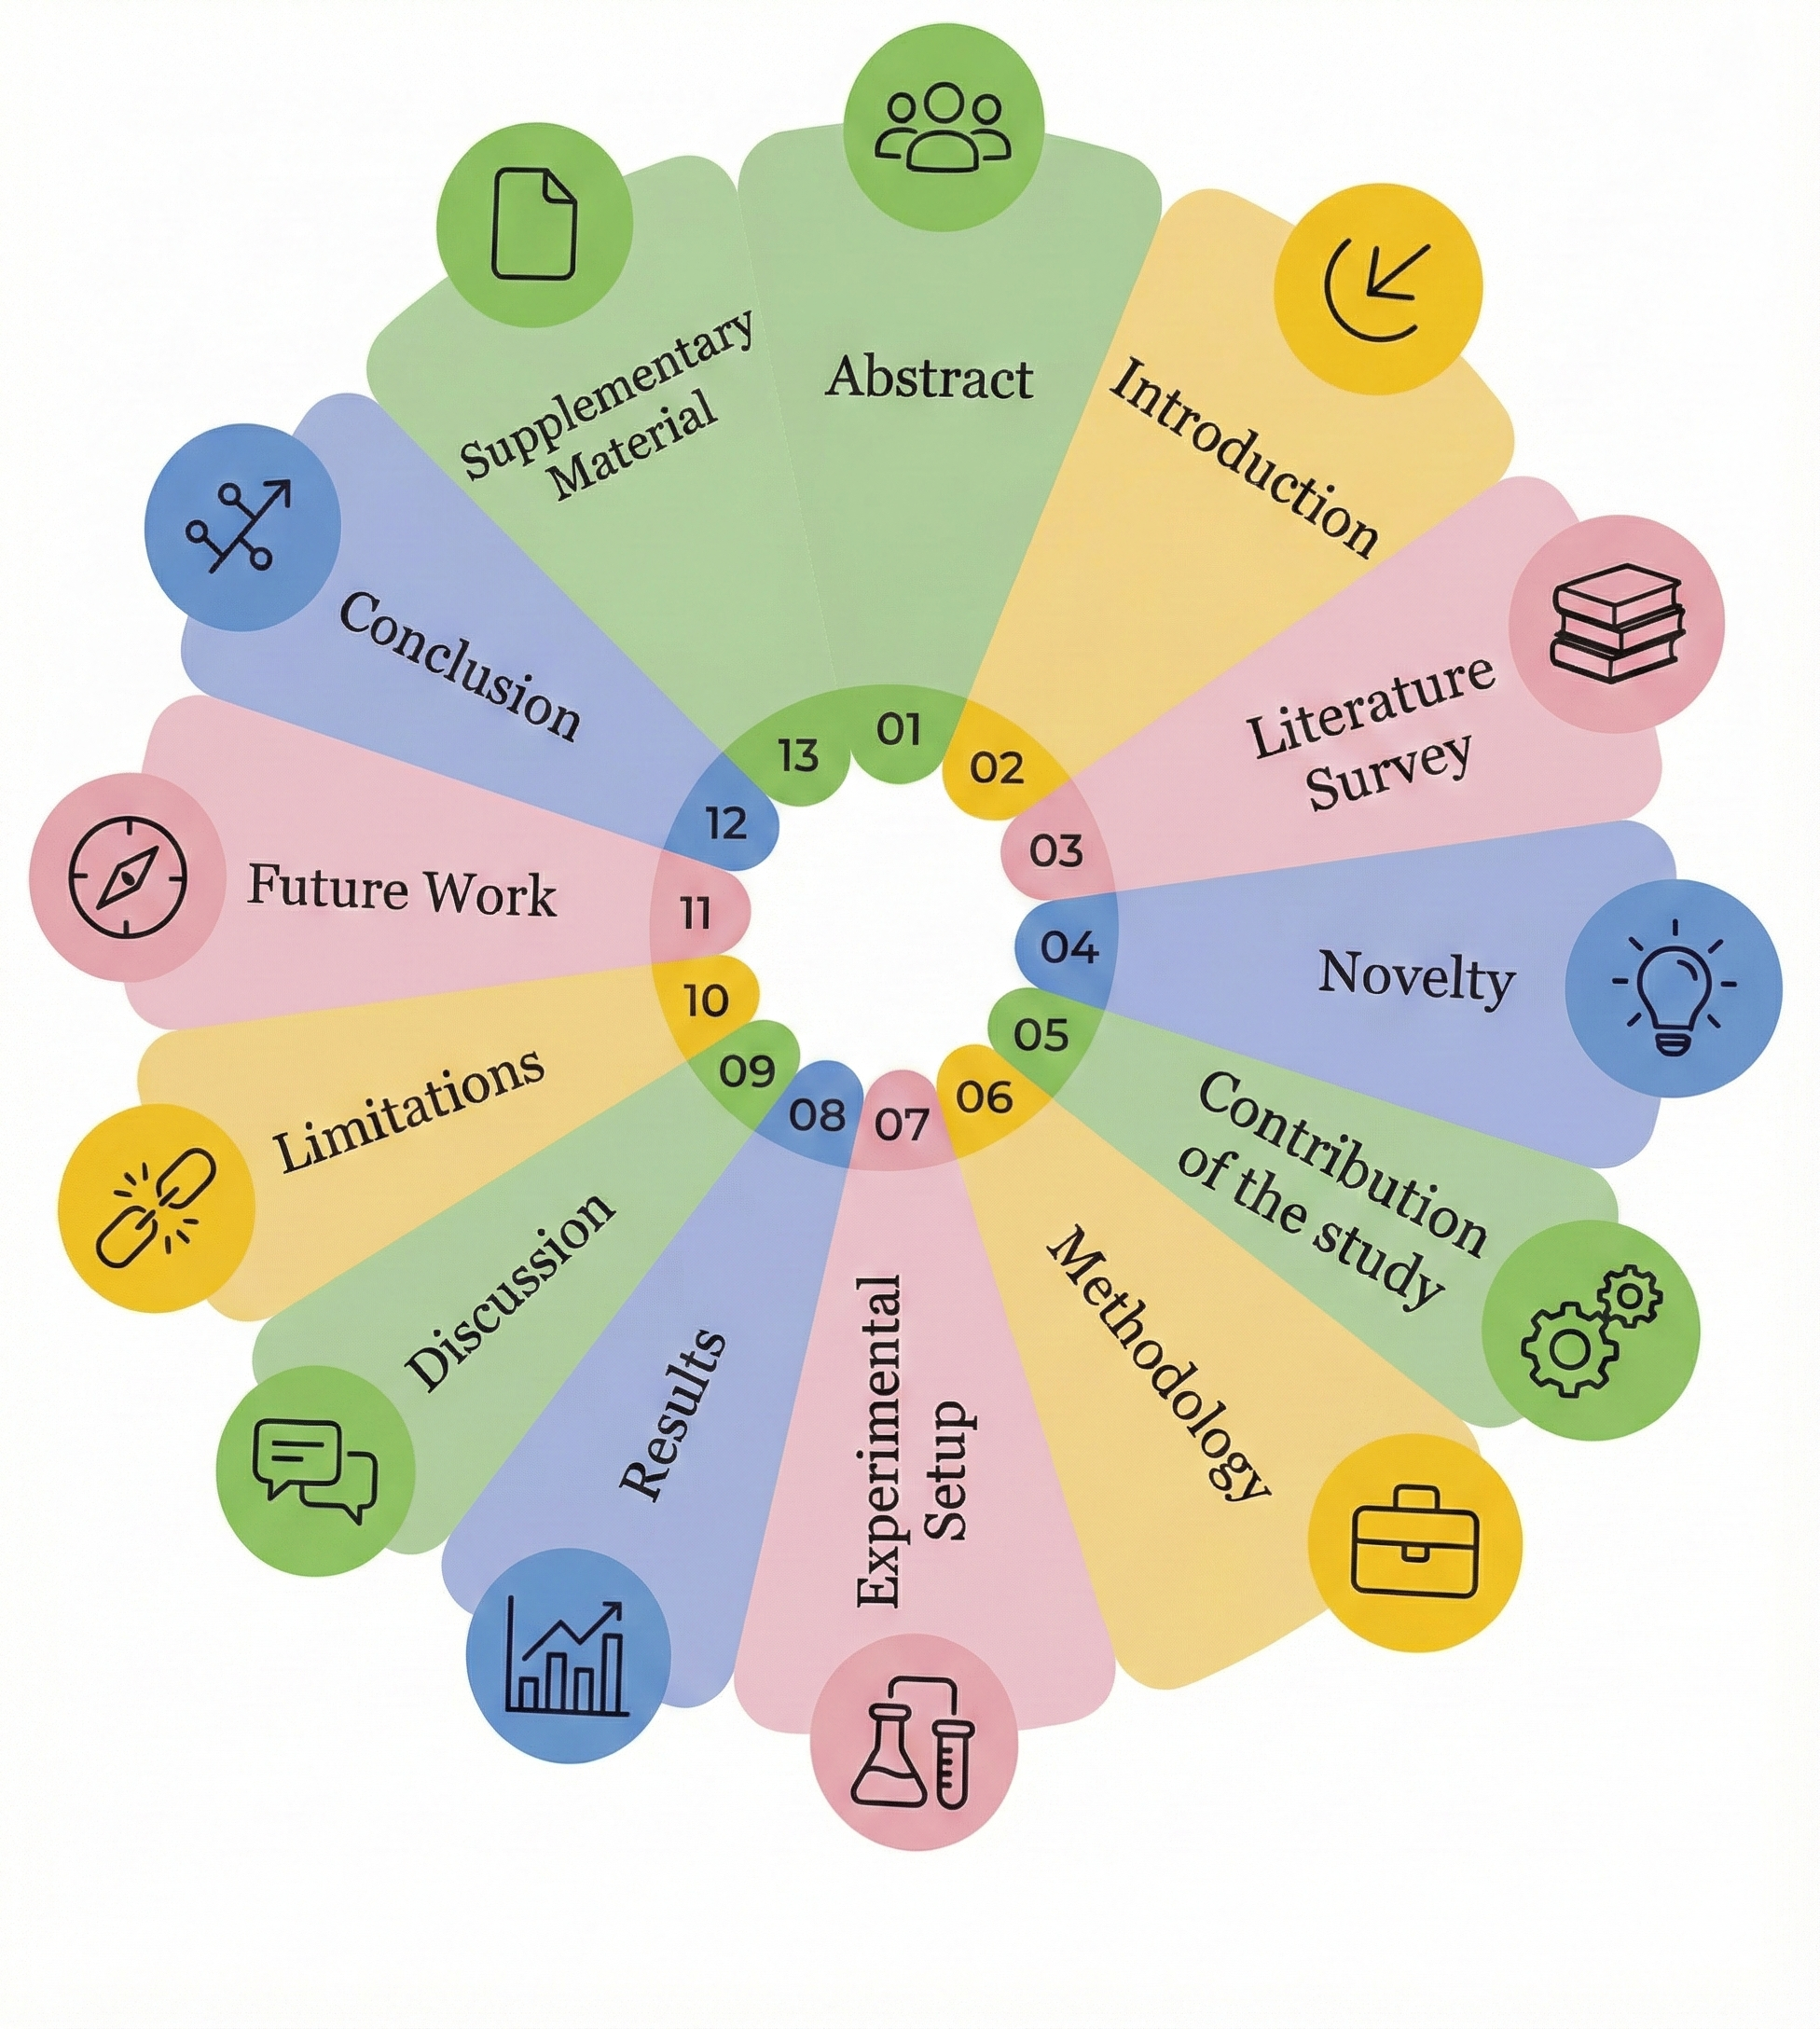
\includegraphics[width=0.75\linewidth]{images/structure_of_the_study.png}
		\caption{Structure of the study}
		\label{fig:structure}
	\end{figure}
	
	\section{Literature Survey}\label{sec:literature}
	
	\subsection{Foundational Voice Biomarker Studies}
	
	The application of speech and vocal biomarkers to measure the Parkinson disease (PD) has its roots in the initial studies on dysphonia analysis and irregular speech dynamics. Little et al. showed that nonlinear recurrence structures and fractal scaling properties of the sustained phonation signals can be used to characterize pathological voice disorders that are a result of Parkinsonian dysarthria \cite{little-2007}. This study formed one of the first quantitative correlations between the abnormalities in the acoustic signals and the neurodegenerative motor disabilities.
	
	Later validation research showed that dysphonia measurements were appropriate to remote clinical monitoring. Later on, Little et al. demonstrated that the acoustic perturbation measures derived during sustained phonation are stable and clinically informative in the telemonitoring environment, demonstrating the possibility of management of diseases continuously and without the need to be invasive \cite{little-2008}. Based on these results, Tsanas et al. proposed a milestone in telemonitoring framework, where the speech derived acoustic features were directly mapped onto Unified Parkinson Disease Rating Scale (UPDRS) scores with regression modelling, showing that they can accurately estimate the severity of the disease in non-clinical settings \cite{tsanas-2009}.
	
	Parallel clinical studies highlighted the significance of dependable biomarkers that can help in the process of describing heterogeneous disease progression. Research into markers of PD progression found that speech features were scalable complements of the conventional neurological assessment \cite{maetzler-2009}. Subsequent machine learning prognostic models investigated rapid disease progression baseline prediction, and this support was given to the clinical significance of quantitative biomarkers \cite{tsiouris-2017}.
	
	The development of digital health and computational phenotyping further stimulated the interest in voice analysis as a goal neurological biomarker. In-depth phenotyping studies were able to point out speech cues as expressive representations of motor, cognitive, and emotional disability among PD patients \cite{tracy-2019}. The results of comparative studies on several speech datasets showed that the acoustic biomarkers are generalizable in different recording conditions and populations \cite{neto-2024}. There is also recent machine learning research that has proven voice analysis to be valuable in application in the context of early intervention and screening \cite{swain-2024}.
	
	In addition to motor impairment, it has also been demonstrated that Parkinsonian speech is accompanied by emotional and prosodic dysfunctions which can be revealed by the analysis of machine learning and advocate the idea of multidimensional diagnostic use of speech \cite{sechidis-2021}. Explainable speech-based diagnostic models have later focused on visibility and clinical reliability in non-invasive PD diagnostic systems \cite{xu-2025}.
	
	Extensive literature reviews have always listed speech analysis among the most advanced digital biomarkers of monitoring and progression measurement of Parkinson disease \cite{jasim-2025,hossain-2025}. These reviews highlight reliability, scalability of voice-based assessment and non-invasiveness of voice-based assessment in clinical and telehealth settings.
	
	The outlook of more recent systematic reviews also underlines the rapid increase in machine learning and deep learning techniques used to extract speech-based Parkinson-derived biomarkers, which indicates their clinical fullness and the maturity of research  \cite{shokrpour-2025,rabie-2025}. All these papers do prove that voice-based assessment is an established paradigm, which encourages further research to enhance the predictive modeling strategies but not to question the appropriateness of the given modality.
	
	\subsection{Classical Machine Learning and Ensemble Approaches}
	
	Since the introduction of speech cues as credible biomarkers of the presence and severity of Parkinson disease, more and more studies devoted their attention to predictive modeling of the disease state and severity based on classical machine learning methods. Early intelligent systems had operated statistical learning with heuristic optimization to enhance the diagnostic performance. The concept of integrating heterogeneous learning strategy as suggested by Cai et al. has shown the possibilities of making hybrid intelligent framework that incorporates various computational paradigms in predicting Parkinson disease \cite{cai-2017}.
	
	The later research indicated that individual predictive models tend not to characterize the nonlinear and heterogeneous nature of Parkinsonian speech. Ensemble learning methods thus became a natural development in order to enhance robustness and generalization. Nilashi et al. showed that ensemble-based models are much more effective than individual learners in terms of predicting progression because they combine complementary decision boundaries \cite{nilashi-2016,nilashi-2022}.
	
	A number of ensemble architectures were subsequently designed to be used in speech-based severity estimation. Rotation Forest-based ensembles used both variety among base learners to enhance regression stability and prediction performance \cite{sheikhi-2022}. The use of ensemble regression models to predict motor UPDRS also supported that the joint use of predictors results in better performance compared to univariate models \cite{shastry-2023}. It was also demonstrated that hybrid pipelines with an optimized feature selection mechanism can enhance the accuracy of early-stage severity predictions \cite{motamedi-2025,masood-2021}.
	
	New research ventured into more advanced ensemble models such as stacked learning and neuro-fuzzy combinations of New Parkinson disease detection and progression modeling \cite{zhao-2024,omodunbi-2025}. Ensemble learning systems based on vocal features have also been shown to be more reliable in a diagnostic degree in a wide array of datasets and recording conditions \cite{chakole-2025,hassan-2023}.
	
	Based on these advances, our earlier ensemble learning framework proposed a single predictive framework that combined various machine learning models to predict the severity of Parkinson disease \cite{dasgupta-2025}. The paper has shown that heterogeneous model collaboration is beneficial by enhancing the robustness of modeling speech-derived clinical scores with the combination of linear, tree-based, and nonlinear predictors.
	
	Although the effectiveness of ensemble methods has been demonstrated, the vast majority of the available methods assume fixed aggregation techniques, such as averaging, voting or stacking. These fixed combinations are not dynamically adjusted to expert contributions on a case-by-case basis, which may be problematic in terms of specialization such as in the modeling of heterogeneous manifestations of diseases. This drawback inspires the search of the adaptive ensemble paradigms that can input-dependent weighting of experts.
	
	\subsection{Deep Learning and Explainable Modeling}
	
	The quick development of deep learning has had a great impact on the analysis of Parkinson disease, which allows the automatic extraction of the complex representation of speech signals. DNN models have proven to be effective in identifying Parkinsonian speech patterns and estimating the level of the disease without any massive handcrafted feature engineering. Initial deep learning models were based on the idea of enhancing the classification quality based on the learned acoustic representation and tonal analysis models \cite{reddy-2024}.
	
	Recent works have suggested unified deep learning ensemble models of convolutional and sequential networks, in both disease detection and motor severity prediction. These techniques view hierarchical feature learning to learn delicate temporal and spectral variations within the Parkinsonian speech signals \cite{khedimi-2025}. Convolutional ensemble models with the use of confidence-based prediction systems have also enhanced robustness in speech-based diagnostic systems \cite{titouni-2026}.
	
	Along with the improvement of performance there has also been interpretability as a key requirement to clinical adoption. Explainable artificial intelligence (XAI) systems seek to give insight into the decision-making of models, which enhances confidence in clinicians in automated diagnostic systems. Explainable ensemble and deep learning models have been created to emphasize influential vocal biomarkers with a competitive predictive accuracy \cite{aladhadh-2025}. Decipherable speech-analysis systems have also focused on attribution of features and differentiated decision-making in the detection of Parkinson disease at earlier stages \cite{simone-2025,xu-2025}.
	
	In addition to the unimodal speech analysis, scholars have looked into multimodal deep learning systems that combine genetic, visual, and heterogeneous clinical data to enhance disease profiling and diagnosis \cite{cao-2025}. Multimodal representation learning strategies and sparse-attention architectures have been shown to have greater potential to model complex neurological variability between groups of patients \cite{datta-2026}. The comparative studies of machine learning paradigms also support the increasing prevalence of deep learning techniques in research on the topic of Parkinson disease as well as point to continuing issues regarding interpretability, data efficiency, and clinical implementation \cite{chaithanya-2025,kumar-2025}.
		
	Even though they possess high representation abilities, deep learning systems usually make use of monolithic predictors where only one model tries to describe all data variations at once. This design can be a constraint in the face of specialization in the modeling of heterogeneous disease progression patterns. As a result, in the recent past, there has been focus in studies into adaptive and modular learning paradigms that can dynamically distribute predictive responsibility among specialized components, an impetus to embrace Mixture of Experts architecture.

	\subsubsection{Mixture of Experts and Adaptive Modeling}
	
	Mixture of Experts (MoE) architectures are an adaptive paradigm of learning whereby there is a set of specialized models also known as experts which are dynamically combined via a gating mechanism that provides input dependent weights. In contrast to classical ensemble learning based on predetermined aggregation rules, MoE based on conditional computation, different experts can focus on different parts of the data distribution.
	
	The recent developments in machine learning on a large scale have shown the efficiency of MoE systems in working with heterogeneous and high-dimensional data. Transformer based MoE models have been used to classify neurological disorders and this has demonstrated that adaptive expert routing can encode multimodal variability in clinical populations \cite{raza-2025}. Likewise, architectures that are directed by MoE have also been studied in medical imaging pipelines, where expert specialization enhances the performance of region-adaptive reconstruction and prediction \cite{wang-2025}. Research on scalable modular learning systems also emphasizes MoE systems as one of the promising directions to the efficient and flexible design of models in complex learning contexts \cite{hadia-2025}.
	
	Statistically, mixture-based regression models have been widely studied as processes of modeling heterogeneous relationships in data. Theoretical studies indicate that finite mixture regression models offer a strong representational flexibility at the cost of parameter proliferation, expert domination and model degeneracy that require the use of suitable regularization strategies \cite{khalili-2013}. The analysis of contextual explanation networks shows how gating mechanisms can be used at the same time to facilitate adaptive prediction, as well as, interpretable decision-making through input characteristics conditioning model behavior \cite{al-shedivat-2020}.
	
	Whereas adaptive expert systems are recently considered in large-scale and multimodal learning problems, they are not yet applied to structured clinical regression problems. Specifically, there have been relatively limited studies to utilize MoE architectures to estimate the severity of speech-based Parkinson disease in specific scenarios, particularly when other clinical outcomes are predicted together. Current methods are mostly classification or unimodal prediction, as opposed to adaptive multi-output regression, based on heterogeneous expert models.
	
	Such observations indicate that there is an apparent avenue of combining adaptive expert specialization and clinically interpretable speech biomarker modeling, which prompts the creation of entropy-regularized Mixture of Experts models to fit Parkinson disease severity prediction.
	
	\subsection{Identified Research Gap}
	
	The literature reviewed shows that there has been significant advancement in modeling of Parkinson disease in the speech-derived biomarkers. Early researchers made voice analysis a valid and non-invasive predictor of the presence and severity of disease, whereas classical machine learning and ensemble techniques demonstrated much higher predictive accuracy upon aggregation of the model. Deep learning techniques also improved the ability of the representation learning and the ability to extract complex acoustic patterns automatically. Irrespective of these improvements, a number of significant limitations have not been addressed.
	
	First, the vast majority of the current ensemble learning models utilize fixed aggregation models, including averaging, voting, or stacked generalization where the relative contributions made by models are constant across all samples. Such methods enhance strength, but fail to reflect the diverse nature of Parkinson disease among different people. Dynamically specialized expert models based on patient specific attributes are not common even in sophisticated ensemble systems. We have shown in our earlier ensemble framework that heterogeneous model collaboration proved effective in predicting severity \cite{dasgupta-2025}; the mechanism of aggregation was set globally, preventing adaptive specialisation of the experts.
	
	Second, the severity of PD is commonly measured with a number of correlated clinical outcomes, specifically $motor\_UPDRS$ and $total\_UPDRS$. Available literature often represents those targets in isolation without combining common information across clinical scores. The adaptive expert allocation-based joint multi-output regression is also a comparatively under-explored area of speech-based Parkinson-related disease modeling.
	
	Third, adaptive mixture-based architectures create issues of expert imbalance and dominance where there is a risk that a set of experts could become a monopoly of predictions in training. Although literature suggests the importance of regularization in mixture regression frameworks \cite{khalili-2013}, there are seldom explicit mechanisms that encourage balanced use of experts to clinical predictive models.
	
	All these constraints point to a discrepancy between conventional ensemble learning and entirely adaptive predictive systems with the capability to model the heterogeneous disease progression. In order to fill this gap, the current paper suggests an entropy-regularized adaptive Mixture of Experts model which dynamically attaches expert weights to input properties, and promotes balanced specialization. The suggested architecture incorporates linear, tree-based, and neural predictors in a single framework and jointly multivariate regression of the severity scores of Parkinson disease in voice-based clinical prediction to enhance the flexibility, explainability, and predictability.
	
	\section{Novelty of the Proposed Work} \label{sec:novelty}
	
	Even though some important progress has been made in modeling Parkinson disease with voice biomarkers, current methods depend largely on fixed aggregation of ensembles, or monolithic deep learning models. What is new about this work is the manner in which it is possible to bridge these paradigms by employing an adaptive learning framework that allows specialized expert dynamics yet still interpretable and clinically relevant.
	
	In contrast to traditional ensemble frameworks, which give a fixed pertinacity to the separate frameworks, the proposed framework presents an entropy-regularized Mixture of Experts (MoE) framework that executes input-dependent expert weighting. This will allow heterogeneous predictors to specialise on patient-specific speech properties and deal with variability in disease presentation.
	
	Moreover, unlike in the case of the previous literature, where clinical severity scores are usually predicted separately, the current research establishes the estimation of Parkinson disease severity as a joint multi-output regression task, which simultaneously predicts both motor UPDRS and total UPDRS. This design takes advantage of inter-target correlations which are not fully exploited in current voice-based predictive systems.
	
	The other new feature is the use of entropy to regularize the gating mechanism and avoid dominance of experts and promotes balanced specialization. By combining linear, tree-based, and neural experts under a unified adaptive framework, the proposed approach advances beyond traditional ensemble learning toward a structured, interpretable, and dynamically adaptive predictive system.
	
	To the best of our knowledge, this study represents one of the first applications of an entropy-regularized adaptive Mixture of Experts architecture for joint multi-output Parkinson’s disease severity prediction using voice biomarkers.
	
	The main novelties of the study are presented in Figure~\ref{fig:novelty}.
	
	\begin{figure}[H]
		\centering
		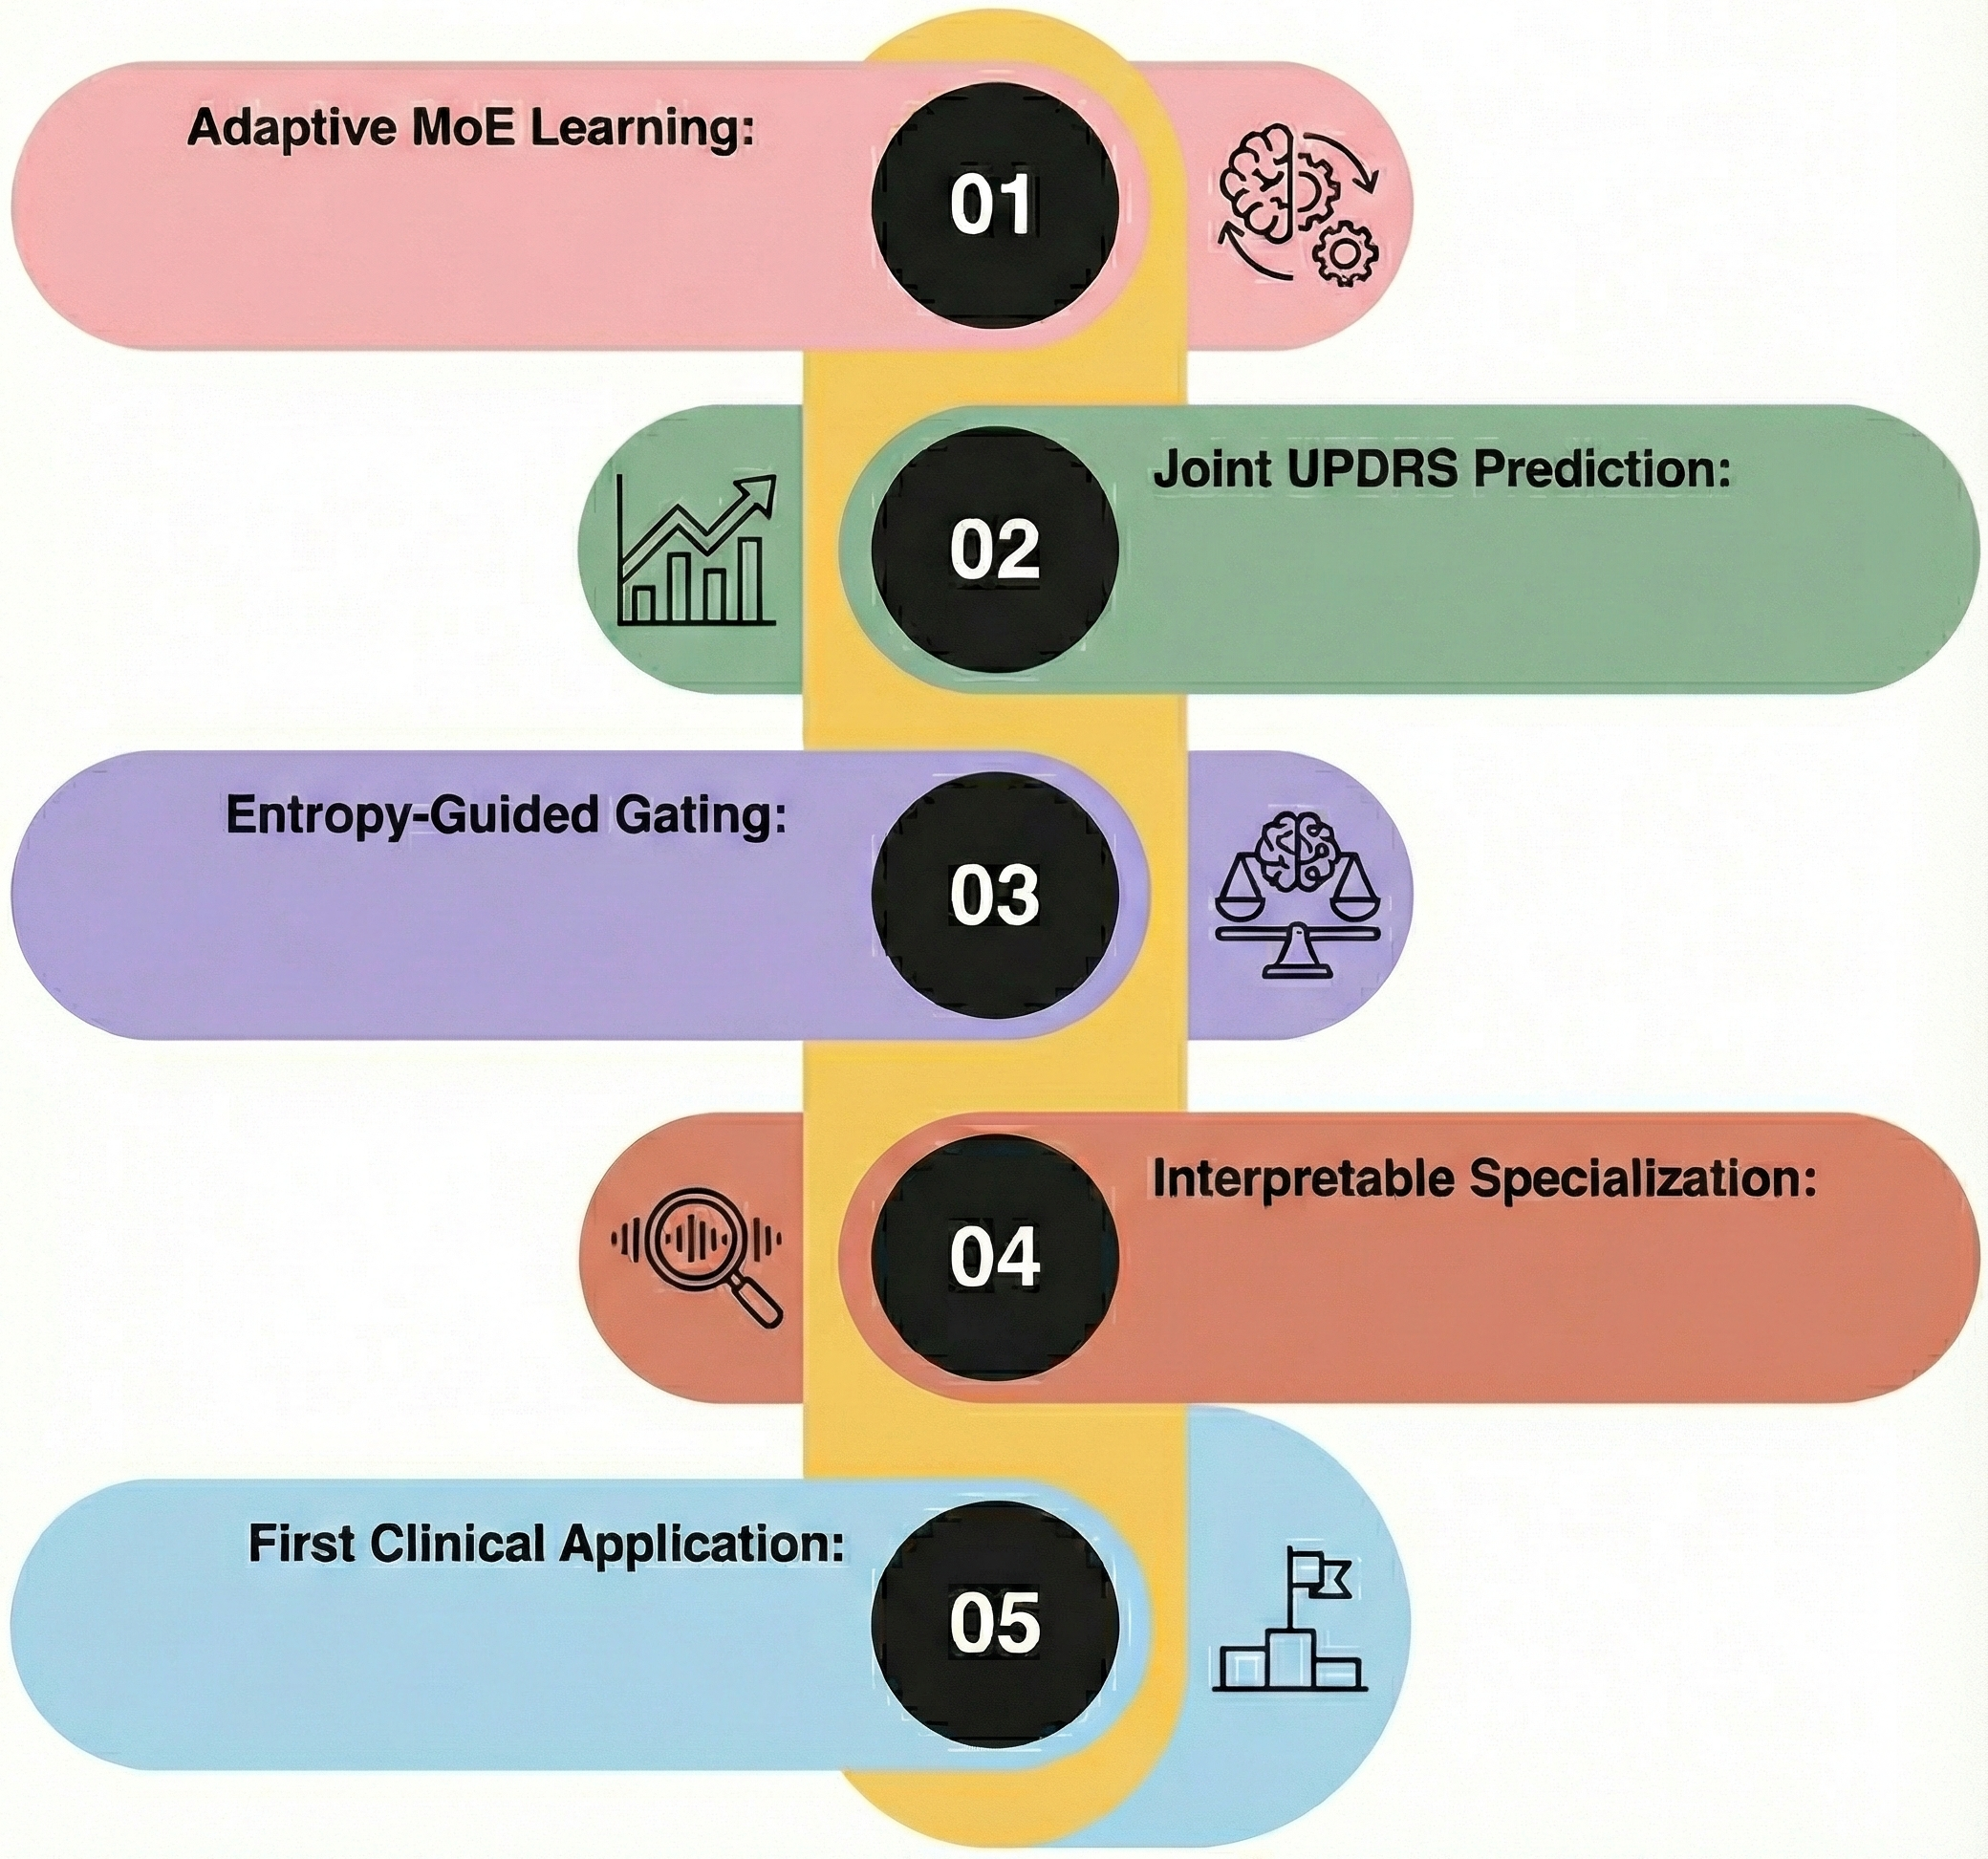
\includegraphics[width=0.75\linewidth]{images/novelty.png}
		\caption{Novelties of the study}
		\label{fig:novelty}
	\end{figure}
	
	\section{Contributions} \label{sec:contributions}
	
	The key findings of this research paper can be summarized as follows:
	
	\begin{enumerate}
		\item Our hypothesis is that an entropy-regularized adaptive Mixture of Experts (MoE) model can be utilized to predict the severity of Parkinsonism-related speech impairment with the help of speech-derived acoustic biomarkers.
		
		\item A target-specific gating mechanism is proposed to dynamically put together heterogeneous expert models, and allows input-dependent specialization in different patient speech patterns.
		
		\item The paper models Parkinson disease severity prediction as a joint multi-output regression problem since the $motor\_UPDRS$ and $total\_UPDRS$ are both estimated at the same time and enables the clinical information to be shared during the learning process.
		
		\item Entropy based regularization approach is integrated in the gating network to avoid expert dominance and encourage balanced use of experts to enhance stability and interpretability of the models.
		
		\item Based on our ensemble framework that was earlier verified \cite{dasgupta-2025}, the proposed architecture brings ensemble learning to expert collaboration through an adaptive mechanism without compromising on reproducibility and transparency.
		
		\item Widespread experimental analysis shows that it has better predictive performance and stability than traditional machine learning, ensemble, and deep learning references.
	\end{enumerate}
	
	\section{Methodology}\label{sec:methodology}
	
	\subsection{Problem Formulation}
	
	We formulate Parkinson’s disease severity prediction as a supervised multi-output regression problem. Let the dataset be defined as
	\begin{equation}
		\mathcal{D} = \{(\mathbf{x}_i, \mathbf{y}_i)\}_{i=1}^{N},
	\end{equation}
	where $\mathbf{x}_i \in \mathbb{R}^{d}$ represents the $d$-dimensional voice feature vector for the $i$-th sample. These features encode acoustic perturbation, noise characteristics, and nonlinear vocal dynamics.
	
	The corresponding multi-target output is defined as
	\begin{equation}
		\mathbf{y}_i =
		\begin{bmatrix}
			y_i^{(m)} \\
			y_i^{(t)}
		\end{bmatrix},
	\end{equation}
	where $y_i^{(m)}$ and $y_i^{(t)}$ denote the $motor\_UPDRS$ and $total\_UPDRS$ scores, respectively.
	
	The objective is to learn a predictive mapping
	\begin{equation}
		f: \mathbb{R}^{d} \rightarrow \mathbb{R}^{2},
	\end{equation}
	that jointly minimizes prediction error for both severity measures. Rather than modeling the two targets independently, we adopt a shared modeling strategy to exploit potential interdependence between motor and total severity scores.
	
	
	\subsection{Heterogeneous Expert Models}
	
	To capture heterogeneous predictive mechanisms within the data, we introduce a set of $K$ complementary expert models:
	\begin{equation}
		\{ f_k(\mathbf{x}; \theta_k) \}_{k=1}^{K},
	\end{equation}
	where $\theta_k$ denotes the parameters of the $k$-th expert.
	
	Each expert produces a two-dimensional prediction:
	\begin{equation}
		\hat{\mathbf{y}}_{i,k} = f_k(\mathbf{x}_i).
	\end{equation}
	
	The expert set includes neural, tree-based, and regularized linear regressors. 
	These models possess fundamentally different inductive biases: neural networks capture nonlinear feature interactions, tree ensembles model hierarchical partitioning of the feature space, and linear models provide regularized parametric baselines. 
	
	Instead of depending on a single global hypothesis class, the framework attempts to exploit complementary representational capabilities by bringing together heterogeneous experts.
	
	\subsection{Adaptive Gating Mechanism}
	
	It is assumed that expert forecasts are consistently relevant across samples when they are averaged statically. However, there are significant individual differences in the voice features and patterns of disease progression. We implement target-specific adaptive gating mechanisms that dynamically allocate expert weights for every sample in order to accommodate this variation.
	
	Two gating functions are defined:
	\begin{equation}
		\mathbf{w}_i^{(m)} = g^{(m)}(\mathbf{x}_i; \phi_m),
	\end{equation}
	\begin{equation}
		\mathbf{w}_i^{(t)} = g^{(t)}(\mathbf{x}_i; \phi_t),
	\end{equation}
	where
	\begin{equation}
		\mathbf{w}_i^{(m)} = [w_{i,1}^{(m)}, \dots, w_{i,K}^{(m)}],
	\end{equation}
	\begin{equation}
		\mathbf{w}_i^{(t)} = [w_{i,1}^{(t)}, \dots, w_{i,K}^{(t)}].
	\end{equation}
	
	Each weight vector is constrained to lie in the probability simplex:
	\begin{equation}
		\sum_{k=1}^{K} w_{i,k}^{(m)} = 1, \quad 
		\sum_{k=1}^{K} w_{i,k}^{(t)} = 1,
	\end{equation}
	\begin{equation}
		w_{i,k}^{(m)} \ge 0, \quad w_{i,k}^{(t)} \ge 0.
	\end{equation}
	
	This convex constraint ensures interpretability and stability, as each prediction becomes a weighted combination of expert outputs.
	
	Final predictions are computed as:
	\begin{equation}
		\hat{y}_i^{(m)} = \sum_{k=1}^{K} w_{i,k}^{(m)} \hat{y}_{i,k}^{(m)},
	\end{equation}
	\begin{equation}
		\hat{y}_i^{(t)} = \sum_{k=1}^{K} w_{i,k}^{(t)} \hat{y}_{i,k}^{(t)}.
	\end{equation}
	
	This formulation enables the model to specialize differently for motor and total severity estimation, allowing distinct expert contributions across targets.
	
	
	\subsection{Entropy Regularization}
	
	Adaptive weighing introduces the possibility of expert dominance, where a single expert gains almost unit weight across samples, although this is the last thing that should be encouraged. Such a collapse reduces the variety and eliminates the benefit of congregation.
	
	Entropy regularization is also used on both gating distributions to give balanced specialization.
	
	The entropy for the motor weights is:
	\begin{equation}
		\mathcal{H}^{(m)} = - \frac{1}{N} 
		\sum_{i=1}^{N} \sum_{k=1}^{K} 
		w_{i,k}^{(m)} \log w_{i,k}^{(m)},
	\end{equation}
	
	and similarly for total severity:
	\begin{equation}
		\mathcal{H}^{(t)} = - \frac{1}{N} 
		\sum_{i=1}^{N} \sum_{k=1}^{K} 
		w_{i,k}^{(t)} \log w_{i,k}^{(t)}.
	\end{equation}
	
	Maximizing entropy encourages smoother weight distributions and mitigates premature specialization during training.
		
	\subsection{Training Objective}
	
	Prediction accuracy is measured using joint mean squared error:
	\begin{equation}
		\mathcal{L}_{MSE} = \frac{1}{N} 
		\sum_{i=1}^{N}
		\left[
		(y_i^{(m)} - \hat{y}_i^{(m)})^2 +
		(y_i^{(t)} - \hat{y}_i^{(t)})^2
		\right].
	\end{equation}
	
	The complete objective integrates prediction fidelity with entropy regularization:
	\begin{equation}
		\mathcal{L}_{total}
		=
		\mathcal{L}_{MSE}
		-
		\lambda
		\left(
		\mathcal{H}^{(m)} + \mathcal{H}^{(t)}
		\right),
	\end{equation}
	where $\lambda > 0$ controls the trade-off between accuracy and diversity.
	
	The negative entropy term encourages distributed expert contributions while preserving predictive performance.
\subsection{Training Protocol}


	Before convergence, the expert models are trained separately on the training split. Freezing of their parameters then follows.
	
	To learn adaptive, target specific weight distributions on the condition of entropy regularization, the gating network is then adjusted by the fixed expert predictions.
	
	All experiments use fixed train-validation-test splits to ensure high reproducibility and prevent data leaks.
	
	\section{Experimental Setup}\label{sec:experiments}
	\subsection{Dataset Description}
	
	The Parkinson Telemonitoring Voice Data present in the UCI machine learning repository \cite{parkinsons_telemonitoring_189} were used to conduct experiments. The dataset is comprised of biomedical voice recordings of patients with Parkinsonism disease performing long-term phonation activities when being under telemonitoring conditions.
	
	The data set is comprised of repeated voice recordings of different subjects over time with both the measurements of the acoustic features as well as the clinical severity scores. The demographic data is contained in each recording and in the form of perturbation, noise, and nonlinear dynamical speech features to measure the Parkinsonian dysphonia.
	
	It presents two clinical outcome variables, which are \textit{motor\_UPDRS} and \textit{total\_UPDRS} which are used to denote severity of the motor symptoms and overall disease severity respectively. These are the regression measurements in the study.
	
	This dataset is especially appropriate in researching the non-invasive severity estimation of the Parkinson disease by machine-learning methods since it is provided with longitudinal voice recordings and standardized clinical annotations.
	
	\subsection{Feature Selection and Preprocessing}
	
	The original data had demographic, temporal and acoustic variables, which included:
	
	\texttt{subject\#, age, sex, test\_time, motor\_UPDRS, total\_UPDRS,}
	\texttt{Jitter(\%), Jitter(Abs), Jitter:RAP, Jitter:PPQ5, Jitter:DDP,}
	\texttt{Shimmer, Shimmer(dB), Shimmer:APQ3, Shimmer:APQ5,}
	\texttt{Shimmer:APQ11, Shimmer:DDA, NHR, HNR, RPDE, DFA, PPE}.
	
	The identifier \texttt{subject\#} was removed as it does not encode predictive information. The temporal index \texttt{test\_time} was also excluded to prevent leakage of longitudinal ordering effects. 
	
	The final feature representation consisted of 18 variables capturing demographic attributes and acoustic perturbation, noise, and nonlinear vocal dynamics.
	
	\subsection{Dataset Partitioning}
	
	The dataset contains $N = 5{,}875$ samples with $d = 18$ features and two regression targets. The partitions are summarized in Table \ref{tab:data_splits}. Fixed splits were maintained across all experiments to ensure strict reproducibility.
	
	\begin{table}[htbp]
		\centering
		\caption{Dataset partition summary}
		\label{tab:data_splits}
		\begin{tabular}{|l|c|c|c|}
			\hline
			Split & Samples & Feature Dim. & Target Dim. \\
			\hline
			Training & 3760 & 18 & 2 \\
			Validation & 940 & 18 & 2 \\
			Test & 1175 & 18 & 2 \\
			\hline
			Total & 5875 & 18 & 2 \\
			\hline
		\end{tabular}
	\end{table}
	
	\subsection{Data Normalization}
	
	All input features and target variables were standardized using z-score normalization to ensure stable optimization across heterogeneous models.
	
	For inputs:
	\[
	\tilde{x}_{ij} = \frac{x_{ij} - \mu_j}{\sigma_j},
	\]
	where statistics were computed exclusively from training data.
	
	Targets were jointly standardized using a separate scaler fitted on the two-dimensional training target matrix:
	\[
	\tilde{\mathbf{y}}_i =
	\frac{\mathbf{y}_i - \boldsymbol{\mu}_y}{\boldsymbol{\sigma}_y}.
	\]
	
	All evaluation metrics were computed after inverse-transforming predictions back to clinical scale.
	
	\subsection{Expert Model Configuration}
	
	Four heterogeneous expert models were independently trained prior to gating optimization.
	
	\subsubsection{Neural Network Expert}
	
	The neural expert is a fully connected feedforward architecture (18–64–64–64–32) with ReLU activations, L2 regularization, and dropout. Optimization was performed using Adam with early stopping.
	
	\begin{table}[htbp]
		\centering
		\caption{Neural Network hyperparameters}
		\label{tab:nn_params}
		\begin{tabular}{|l|c|}
			\hline
			Hyperparameter & Value \\
			\hline
			Hidden Layers & 64–64–64–32 \\
			Activation & ReLU \\
			Dropout & 0.00034 \\
			L2 Regularization & $10^{-4}$ \\
			Optimizer & Adam \\
			Learning Rate & 0.01 \\
			Batch Size & 64 \\
			Max Epochs & 300 \\
			Early Stopping Patience & 50 \\
			\hline
		\end{tabular}
	\end{table}
	
	\subsubsection{Random Forest Expert}
	
	The Random Forest model provides nonlinear partition-based regression with ensemble averaging.
	
	\begin{table}[htbp]
		\centering
		\caption{Random Forest hyperparameters}
		\label{tab:rf_params}
		\begin{tabular}{|l|c|}
			\hline
			Hyperparameter & Value \\
			\hline
			Number of Trees & 400 \\
			Maximum Depth & 40 \\
			Criterion & squared\_error \\
			Bootstrap & True \\
			OOB Score & Enabled \\
			Min Samples Split & 2 \\
			Min Samples Leaf & 1 \\
			\hline
		\end{tabular}
	\end{table}
	
	\subsubsection{Ridge Regression Expert}
	
	The Ridge regression model provides a regularized linear baseline for multi-output regression.
	
	\begin{table}[htbp]
		\centering
		\caption{Ridge Regression hyperparameters}
		\label{tab:ridge_params}
		\begin{tabular}{|l|c|}
			\hline
			Hyperparameter & Value \\
			\hline
			Regularization $\alpha$ & 45.35 \\
			Fit Intercept & True \\
			\hline
		\end{tabular}
	\end{table}
	
	\subsubsection{Elastic Net Expert}
	
	The MultiTaskElasticNetCV model performs joint regression with combined L1–L2 regularization.
	
	\begin{table}[htbp]
		\centering
		\caption{Elastic Net hyperparameters}
		\label{tab:enet_params}
		\begin{tabular}{|l|c|}
			\hline
			Hyperparameter & Value \\
			\hline
			Cross-Validation Folds & 5 \\
			Max Iterations & 5000 \\
			Tolerance & 0.001 \\
			Selection Strategy & cyclic \\
			L1 Ratio Grid & [0.1, 0.3, ...] \\
			\hline
		\end{tabular}
	\end{table}
	
	\subsection{Meta-Feature Construction}
	
	Each expert produces a two-dimensional prediction vector. For $K=4$ experts, their outputs are concatenated to form an 8-dimensional meta-feature vector:
	
	\[
	\mathbf{z}_i \in \mathbb{R}^{8}.
	\]
	
	This representation captures cross-expert predictive patterns and serves as input to the adaptive gating network.
	
	\subsection{Gating Network Architecture}
	
	The gating module is defined as \texttt{MoEGate(input\_dim=8, hidden\_dim=32, n\_experts=4)}. It consists of a single hidden layer with ReLU activation and produces $2 \times 4$ outputs corresponding to target-specific expert weights. Softmax normalization enforces convex constraints.
	
	\begin{table}[H]
		\centering
		\caption{Gating Network hyperparameters}
		\label{tab:gating_params}
		\begin{tabular}{|l|c|}
			\hline
			Hyperparameter & Value \\
			\hline
			Input Dimension & 8 \\
			Hidden Units & 32 \\
			Number of Experts & 4 \\
			Optimizer & Adam \\
			Batch Size & 64 \\
			Max Epochs & 300 \\
			Early Stopping Patience & 50 \\
			Entropy Coefficient $\lambda$ & 0.01 \\
			Training Samples & 4700 \\
			\hline
		\end{tabular}
	\end{table}
	
	Early stopping was triggered at epoch 51 based on validation MSE monitoring.
	
	\subsection{Production Workflow}
	
	The system functions as a modular decision-support pipeline from a production standpoint. Four separate expert modules evaluate voice telemonitoring data once it has been preprocessed and normalized. An adaptive gating engine processes expert outputs, aggregating them into meta-features and calculating target-specific weight distributions. Prior to being sent to the end user, the final severity predictions produced by weighted fusion are inversely converted to clinical scale.
	
	The complete workflow is illustrated in Figure \ref{fig:flowchart}.
	
	\begin{figure}[H]
		\centering
		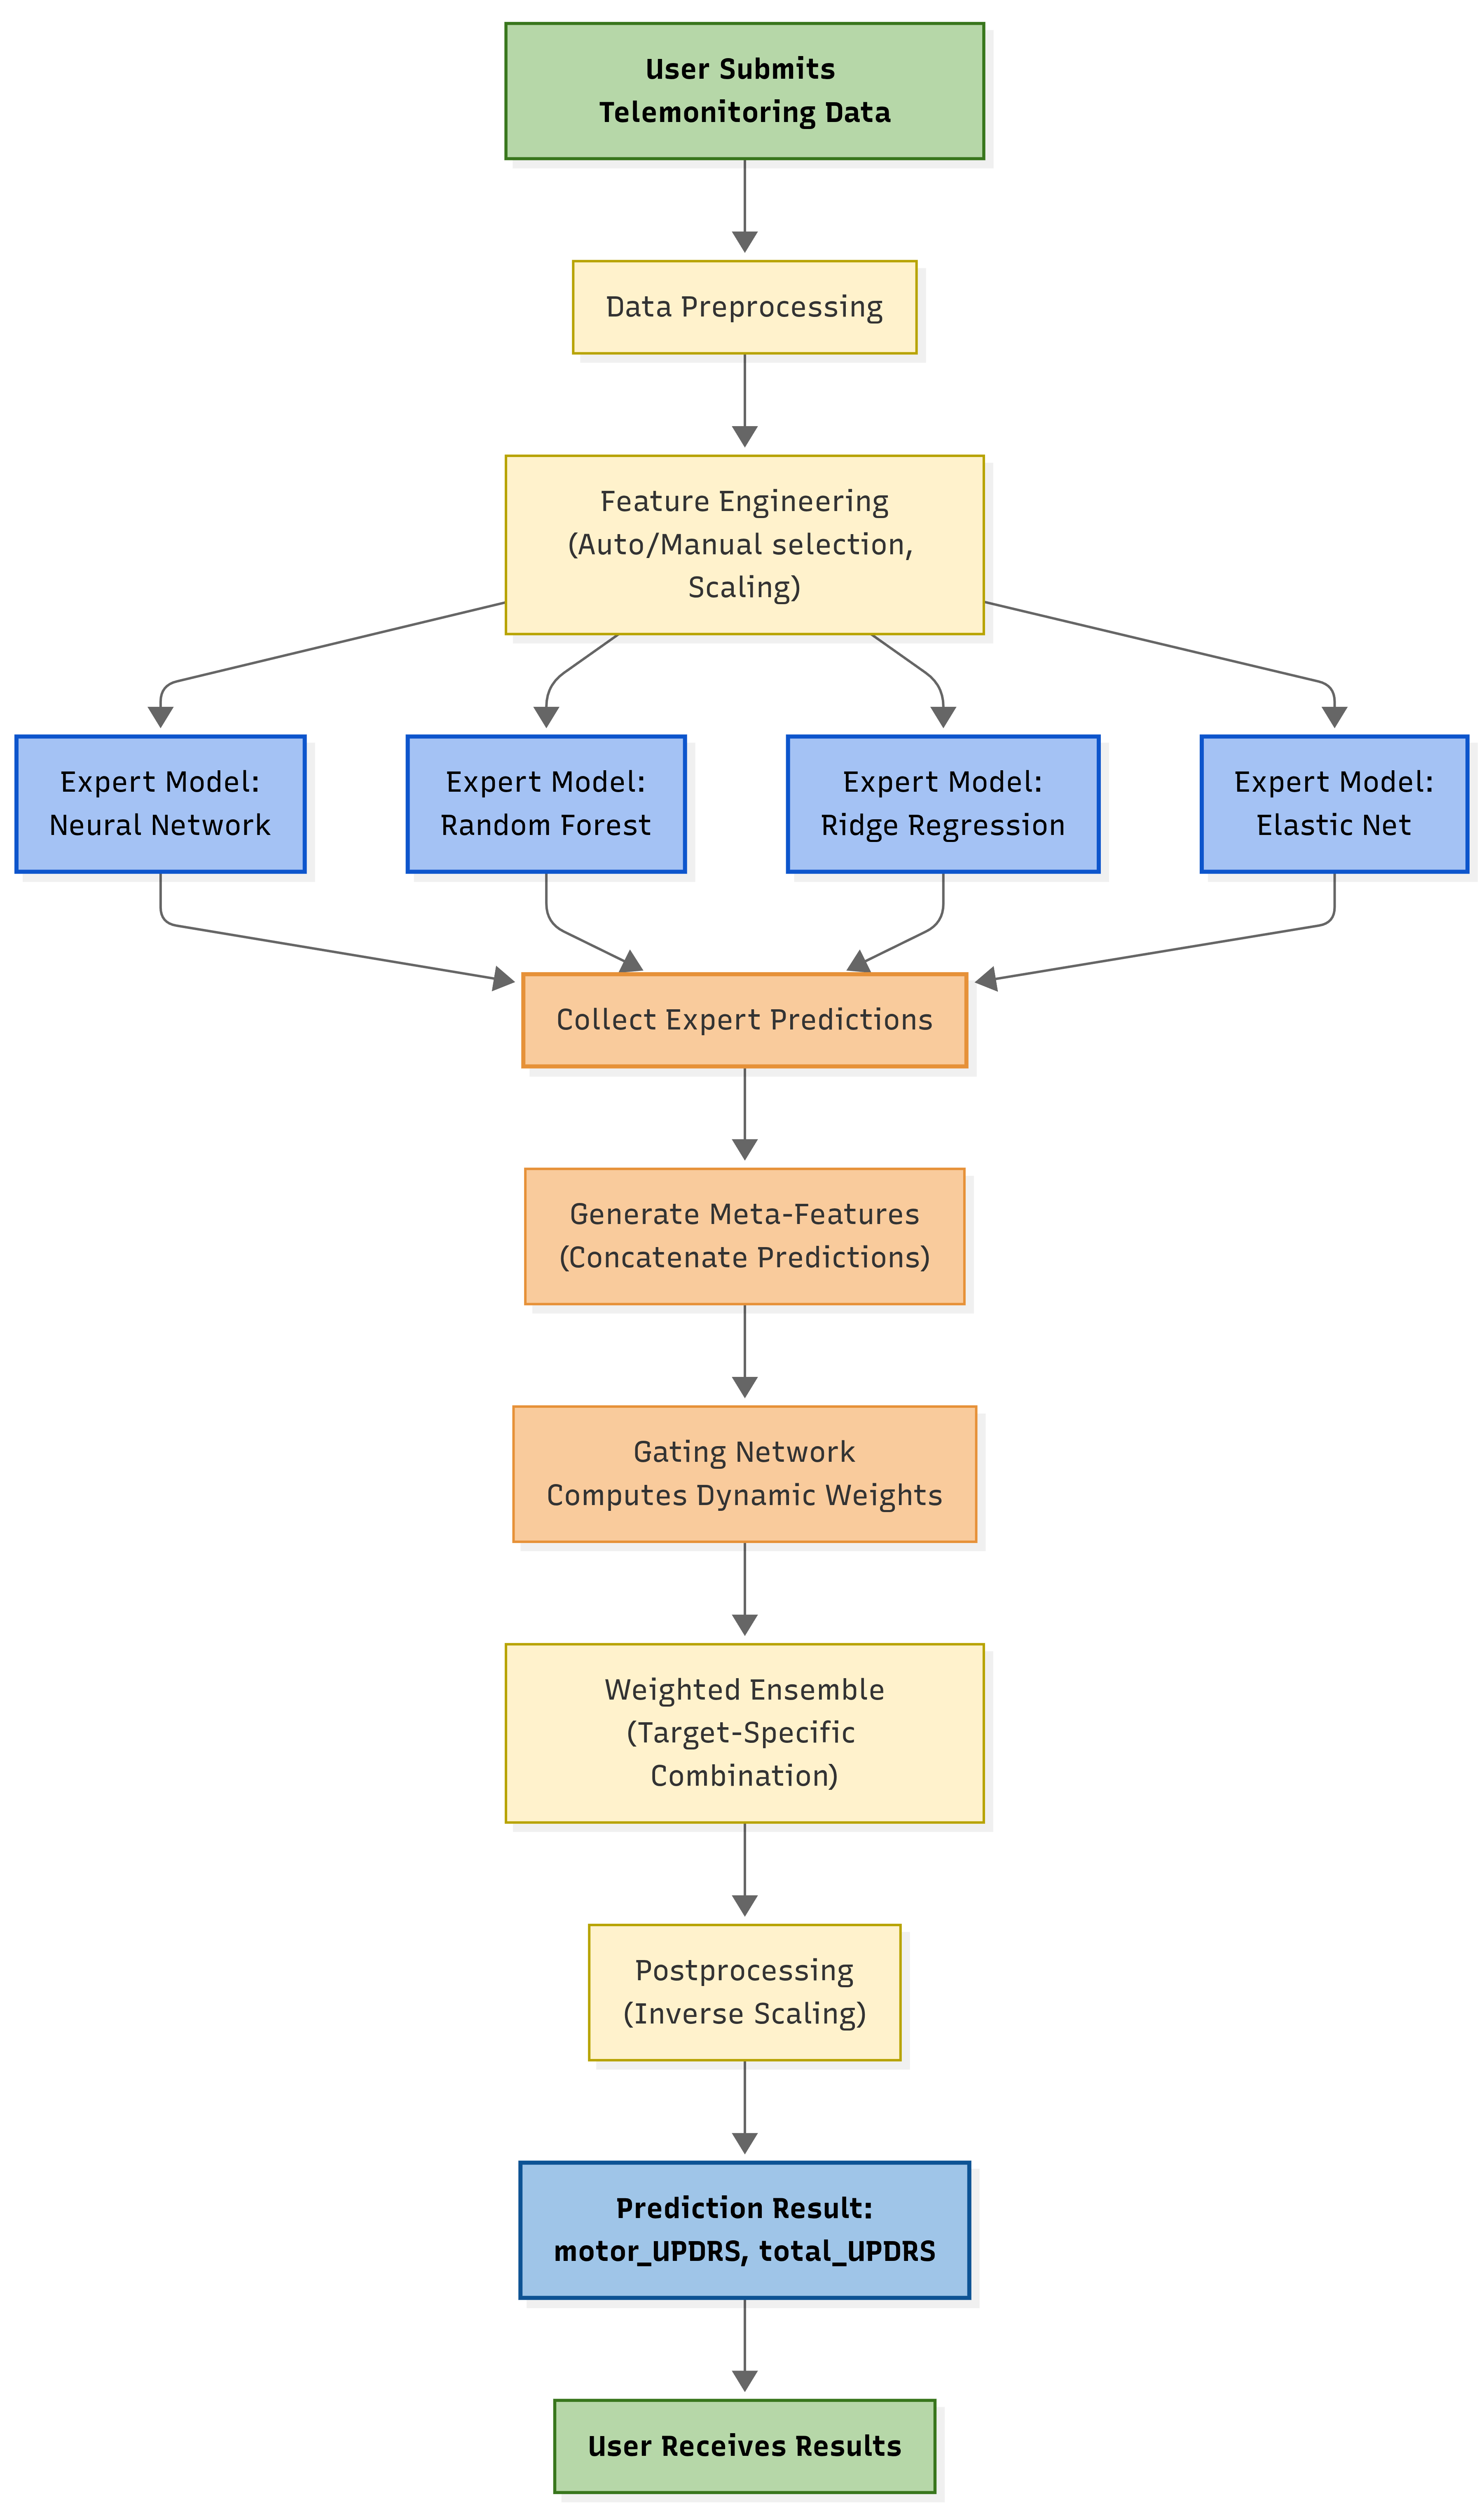
\includegraphics[width=0.75\linewidth]{images/pipeline-flow.png}
		\caption{Production-oriented adaptive Mixture of Experts pipeline.}
		\label{fig:flowchart}
	\end{figure}

	\section{Results}\label{sec:results}

	
	\subsection{Overall Model Performance}
	
	The predictive performance of all models is summarized in Table~\ref{tab:performance_comparison}. The comparison includes coefficient of determination ($R^2$), RMSE, MAE, and MSE computed on the held-out test set.
	
	\begin{table}[htbp]
	\centering
	\caption{Performance comparison of individual experts and the proposed entropy-regularized Mixture of Experts on the test set.}
	\label{tab:performance_comparison}
	\begin{tabular}{lrrrrrr}
		\hline
		Model & Motor $R^2$ & Total $R^2$ & Avg $R^2$ & RMSE & MAE & MSE \\
		\hline
		Random Forest & 0.9131 & 0.9237 & 0.9184 & 2.6457 & 1.9089 & 6.9999 \\
		MoE (Entropy) & 0.9088 & 0.9177 & 0.9133 & 2.7333 & 1.9740 & 7.4710 \\
		Neural Network & 0.8935 & 0.9039 & 0.8987 & 2.9534 & 2.1894 & 8.7228 \\
		Ridge & 0.1157 & 0.1514 & 0.1335 & 8.6743 & 7.2073 & 75.2427 \\
		ElasticNet & 0.1142 & 0.1519 & 0.1331 & 8.6753 & 7.2096 & 75.2605 \\
		\hline
	\end{tabular}
\end{table}
	
	Among all individual experts, the Random Forest achieved the highest predictive performance, with $R^2 = 0.9131$ for $motor\_UPDRS$ and $R^2 = 0.9237$ for $total\_UPDRS$, resulting in an average $R^2$ of 0.9184.
	
	The proposed entropy-regularized Mixture of Experts achieved competitive performance, with $R^2 = 0.9088$ (motor) and $R^2 = 0.9177$ (total). While slightly below the Random Forest in absolute $R^2$, the MoE framework demonstrated improved stability and adaptive weighting behavior across targets.
	
	Neural network performance was moderately strong ($R^2 = 0.8987$ average), whereas linear baselines (Ridge and Elastic Net) exhibited substantially lower explanatory power ($R^2 \approx 0.13$), confirming the nonlinear nature of the mapping between acoustic features and clinical severity.
	
	\subsection{Diagnostic Analysis}
	
	Comparisons of actual-predicted plots indicate that nonlinear ensemble techniques give predictions that closely cluster along the identity line, suggesting that there is high calibration over the severity range. The Random Forest shows the greatest number of concentrations around the diagonal in both of the targets, but the neural network has a slightly larger dispersion at extreme values of severity. These findings are further confirmed by the residual analysis. Random Forest and MoE residuals are centered around zero and have nearly equal dispersion implying that there is not much systematic bias. Linear models on the other hand exhibit organized residual patterns, meaning that they are underfitting and do not represent nonlinear interactions between features. 	Ensemble based models error distributions are approximations of Gaussian behavior with relatively small variance, unlike those of linear models which are heavy tailed.
	
	\subsection{Expert Weight Analysis}
	
	The gating weights learned can be analyzed to show that the Random Forest expert is given dominative average weight to both targets (around 0.92 to motor and 0.88 to total severity). Nevertheless, there is a slightly higher distribution of weighting of total severity prediction among experts and this implies that there is more cross-model complementarity than motor severity estimation. These findings indicate that although tree-based modeling is used to capture most predictive structure, the secondary experts are used to stabilize refinements in certain areas of the feature space.
	
\subsection{Comparative Performance Analysis}

In order to offer a general evaluation of predictive performance with regards to modeling methods, Figure \ref*{fig:model_comparison} offers a comparative visualization of the evaluation measures of all models on the held-out test. It compares both the target-specific and aggregate measures, which makes it possible to directly evaluate the explanatory power and error properties of heterogeneous modeling strategies.

The findings emphasize the benefit of nonlinear ensemble-based practicality in estimating the severity of voice-based Parkinson Disease. The best overall accuracy is obtained by the Random Forest with the proposed entropy-regularized Mixture of Experts coming closely behind. Although tree-based and adaptive models show a significantly better generalization, linear baselines have significantly worse error and low explained variance. Notably, Mixture of Experts framework performs on par with the best single expert and also provides adaptive, target-specific weighting, which makes it interpretable and easy to extend modules beyond fixed ensemble-based approaches.
	
	\begin{figure}[H]
		\centering
		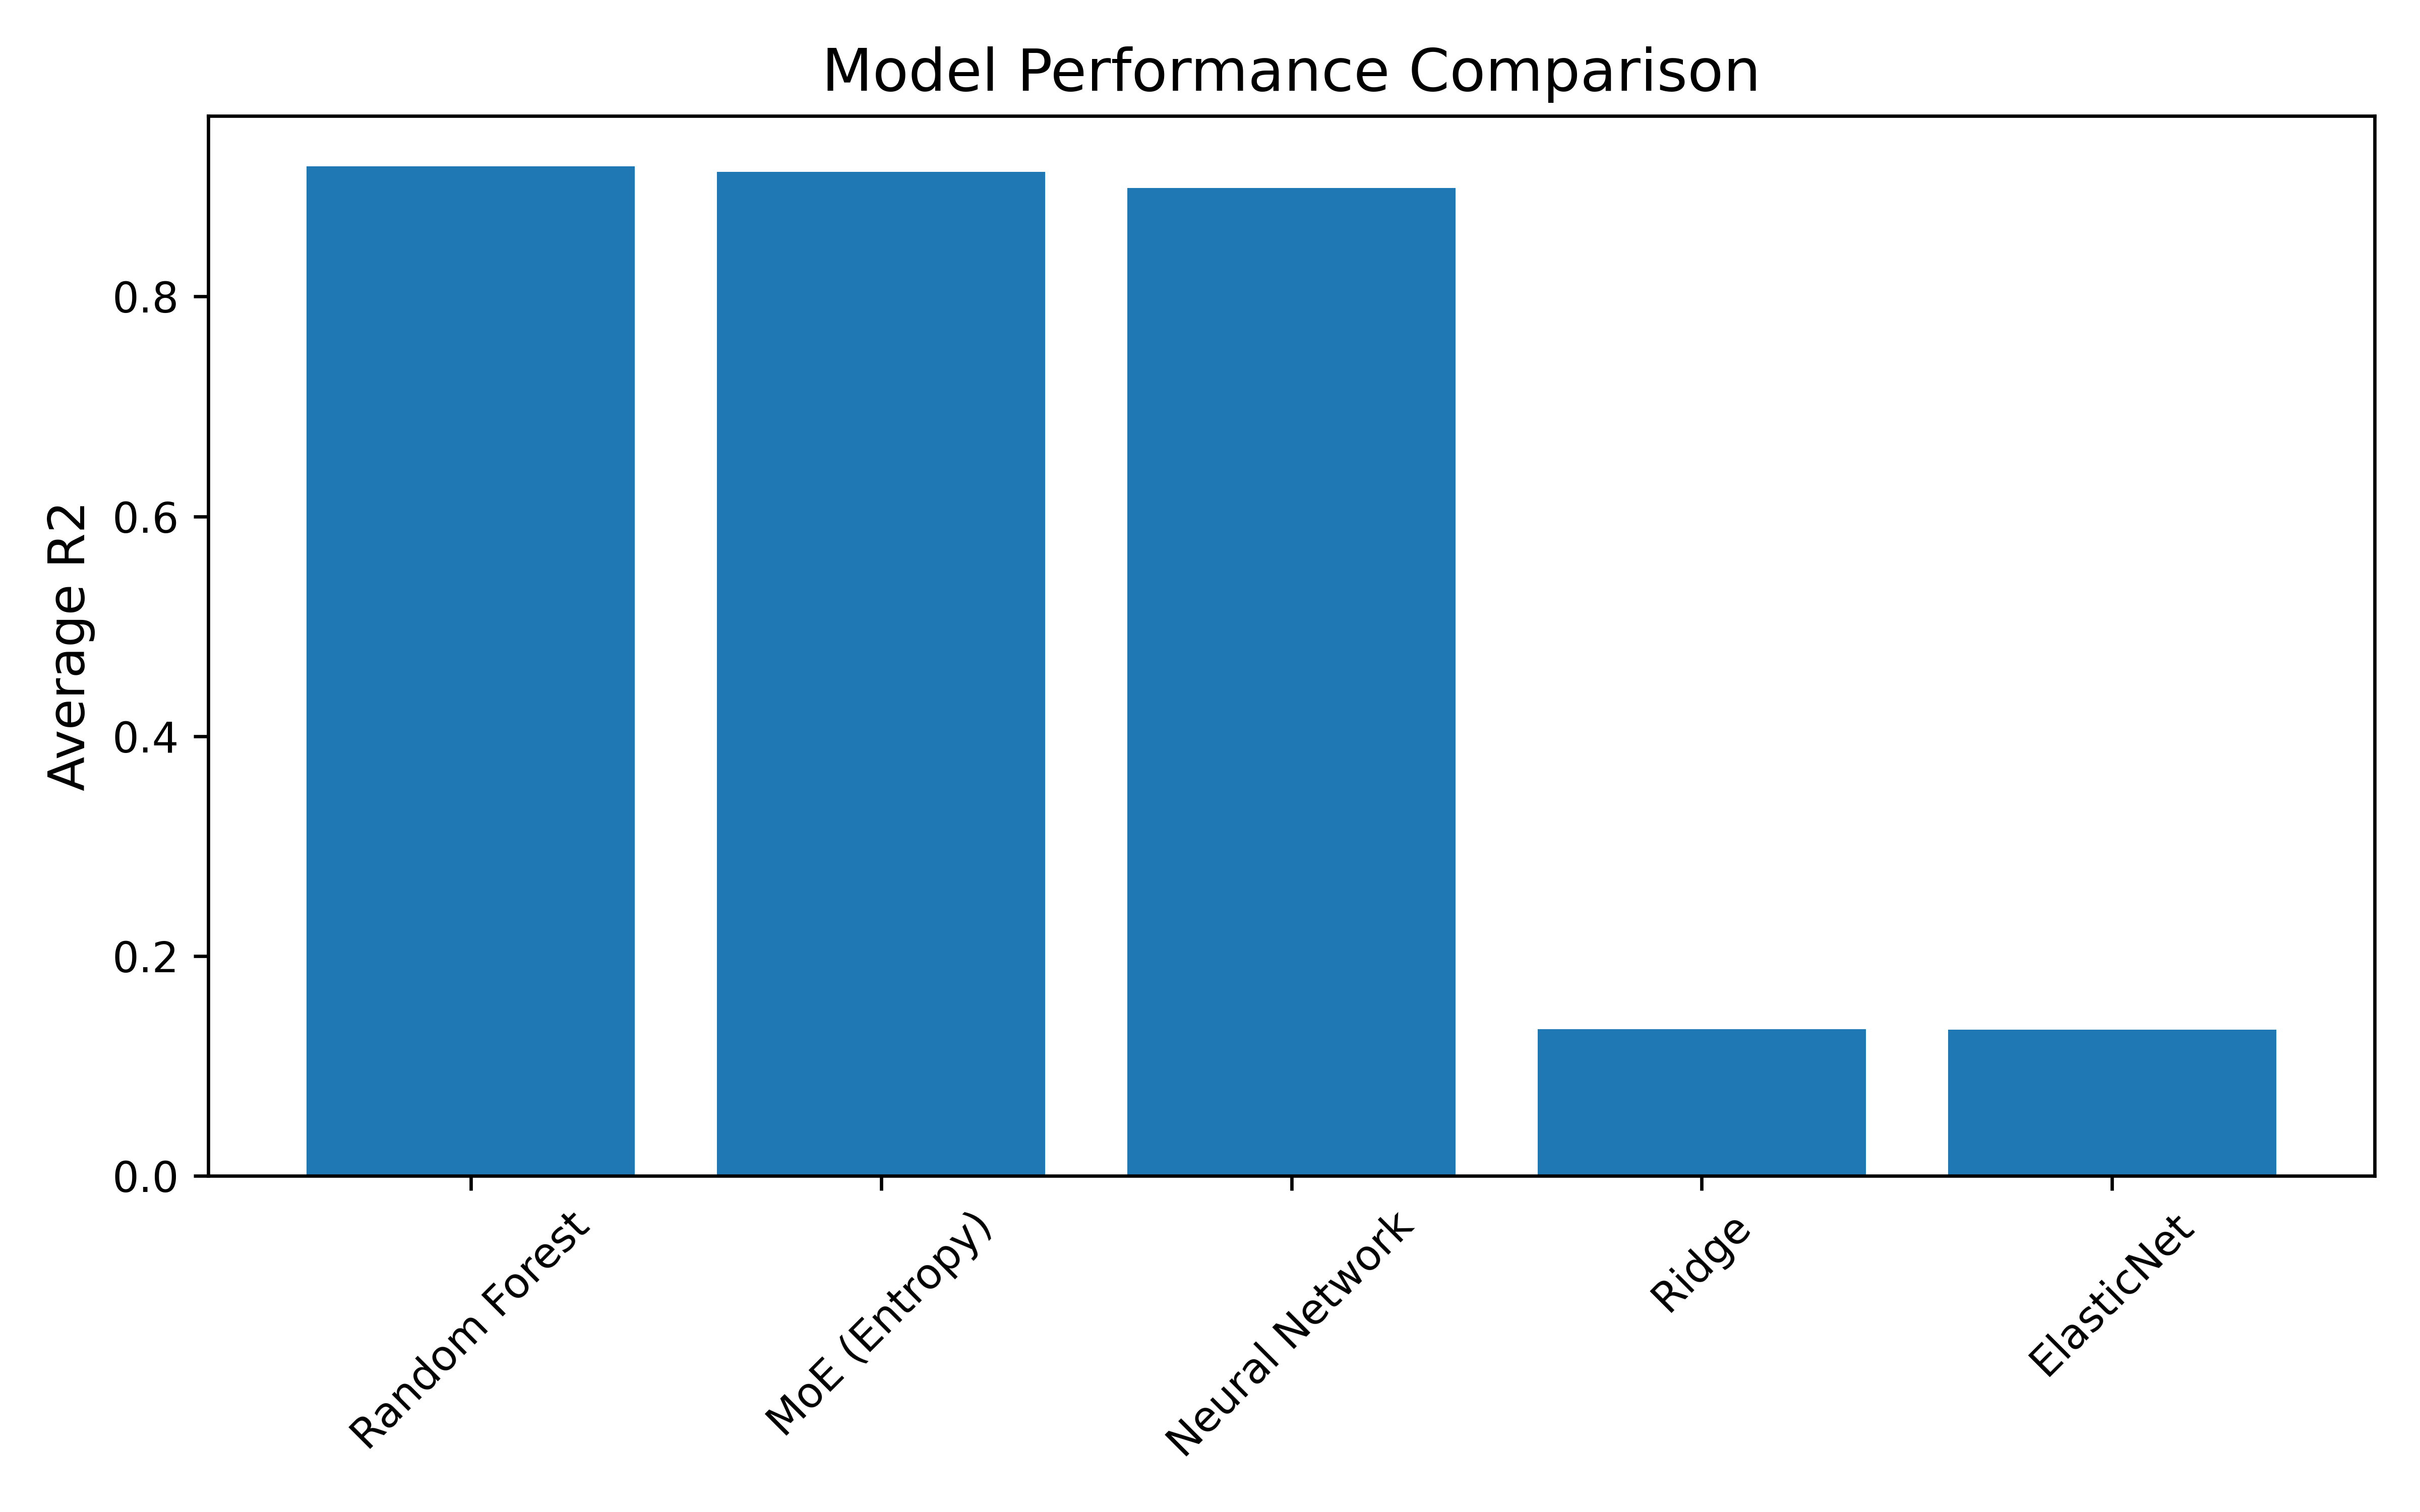
\includegraphics[width=0.8\linewidth]{images/model_performance_comparison.png}
		\caption{Comparative performance of all models across evaluation metrics on the test set.}
		\label{fig:model_comparison}
	\end{figure}
	\subsection{Prediction Calibration and Fit Analysis}
	
	In this attempt to explore more the aspect of predictive behavior without using the aggregate statistics, Figure \ref{fig:actual_vs_pred_main} shows the actual-versus-predicted scatter plots of the two strongest nonlinear models: the proposed entropy-regularized Mixture of Experts and the Random Forest baseline. These plots will give a direct visualization of the quality of calibration of the entire severity range of both $motor\_UPDRS$ and $total\_UPDRS$.	In perfect regression operation, the predictions coincide with the line of identity that suggests that there is correct estimation in low, moderate, and high severity values. The two models have high alignment, which proves their capability of describing nonlinear relationships among acoustic features and clinical outcomes. The random Forest shows a little more clustering around the diagonal and this is expected given that it has slightly higher scores on the $R^2$. The Mixture of Experts, though, can be calibrated competitively and can provide adaptive target-specific weighting, implying that dynamic expert fusion can be used to maintain predictive fidelity with structural interpretability.
	\begin{figure}[H]
		\centering
		\begin{subfigure}{0.45\linewidth}
			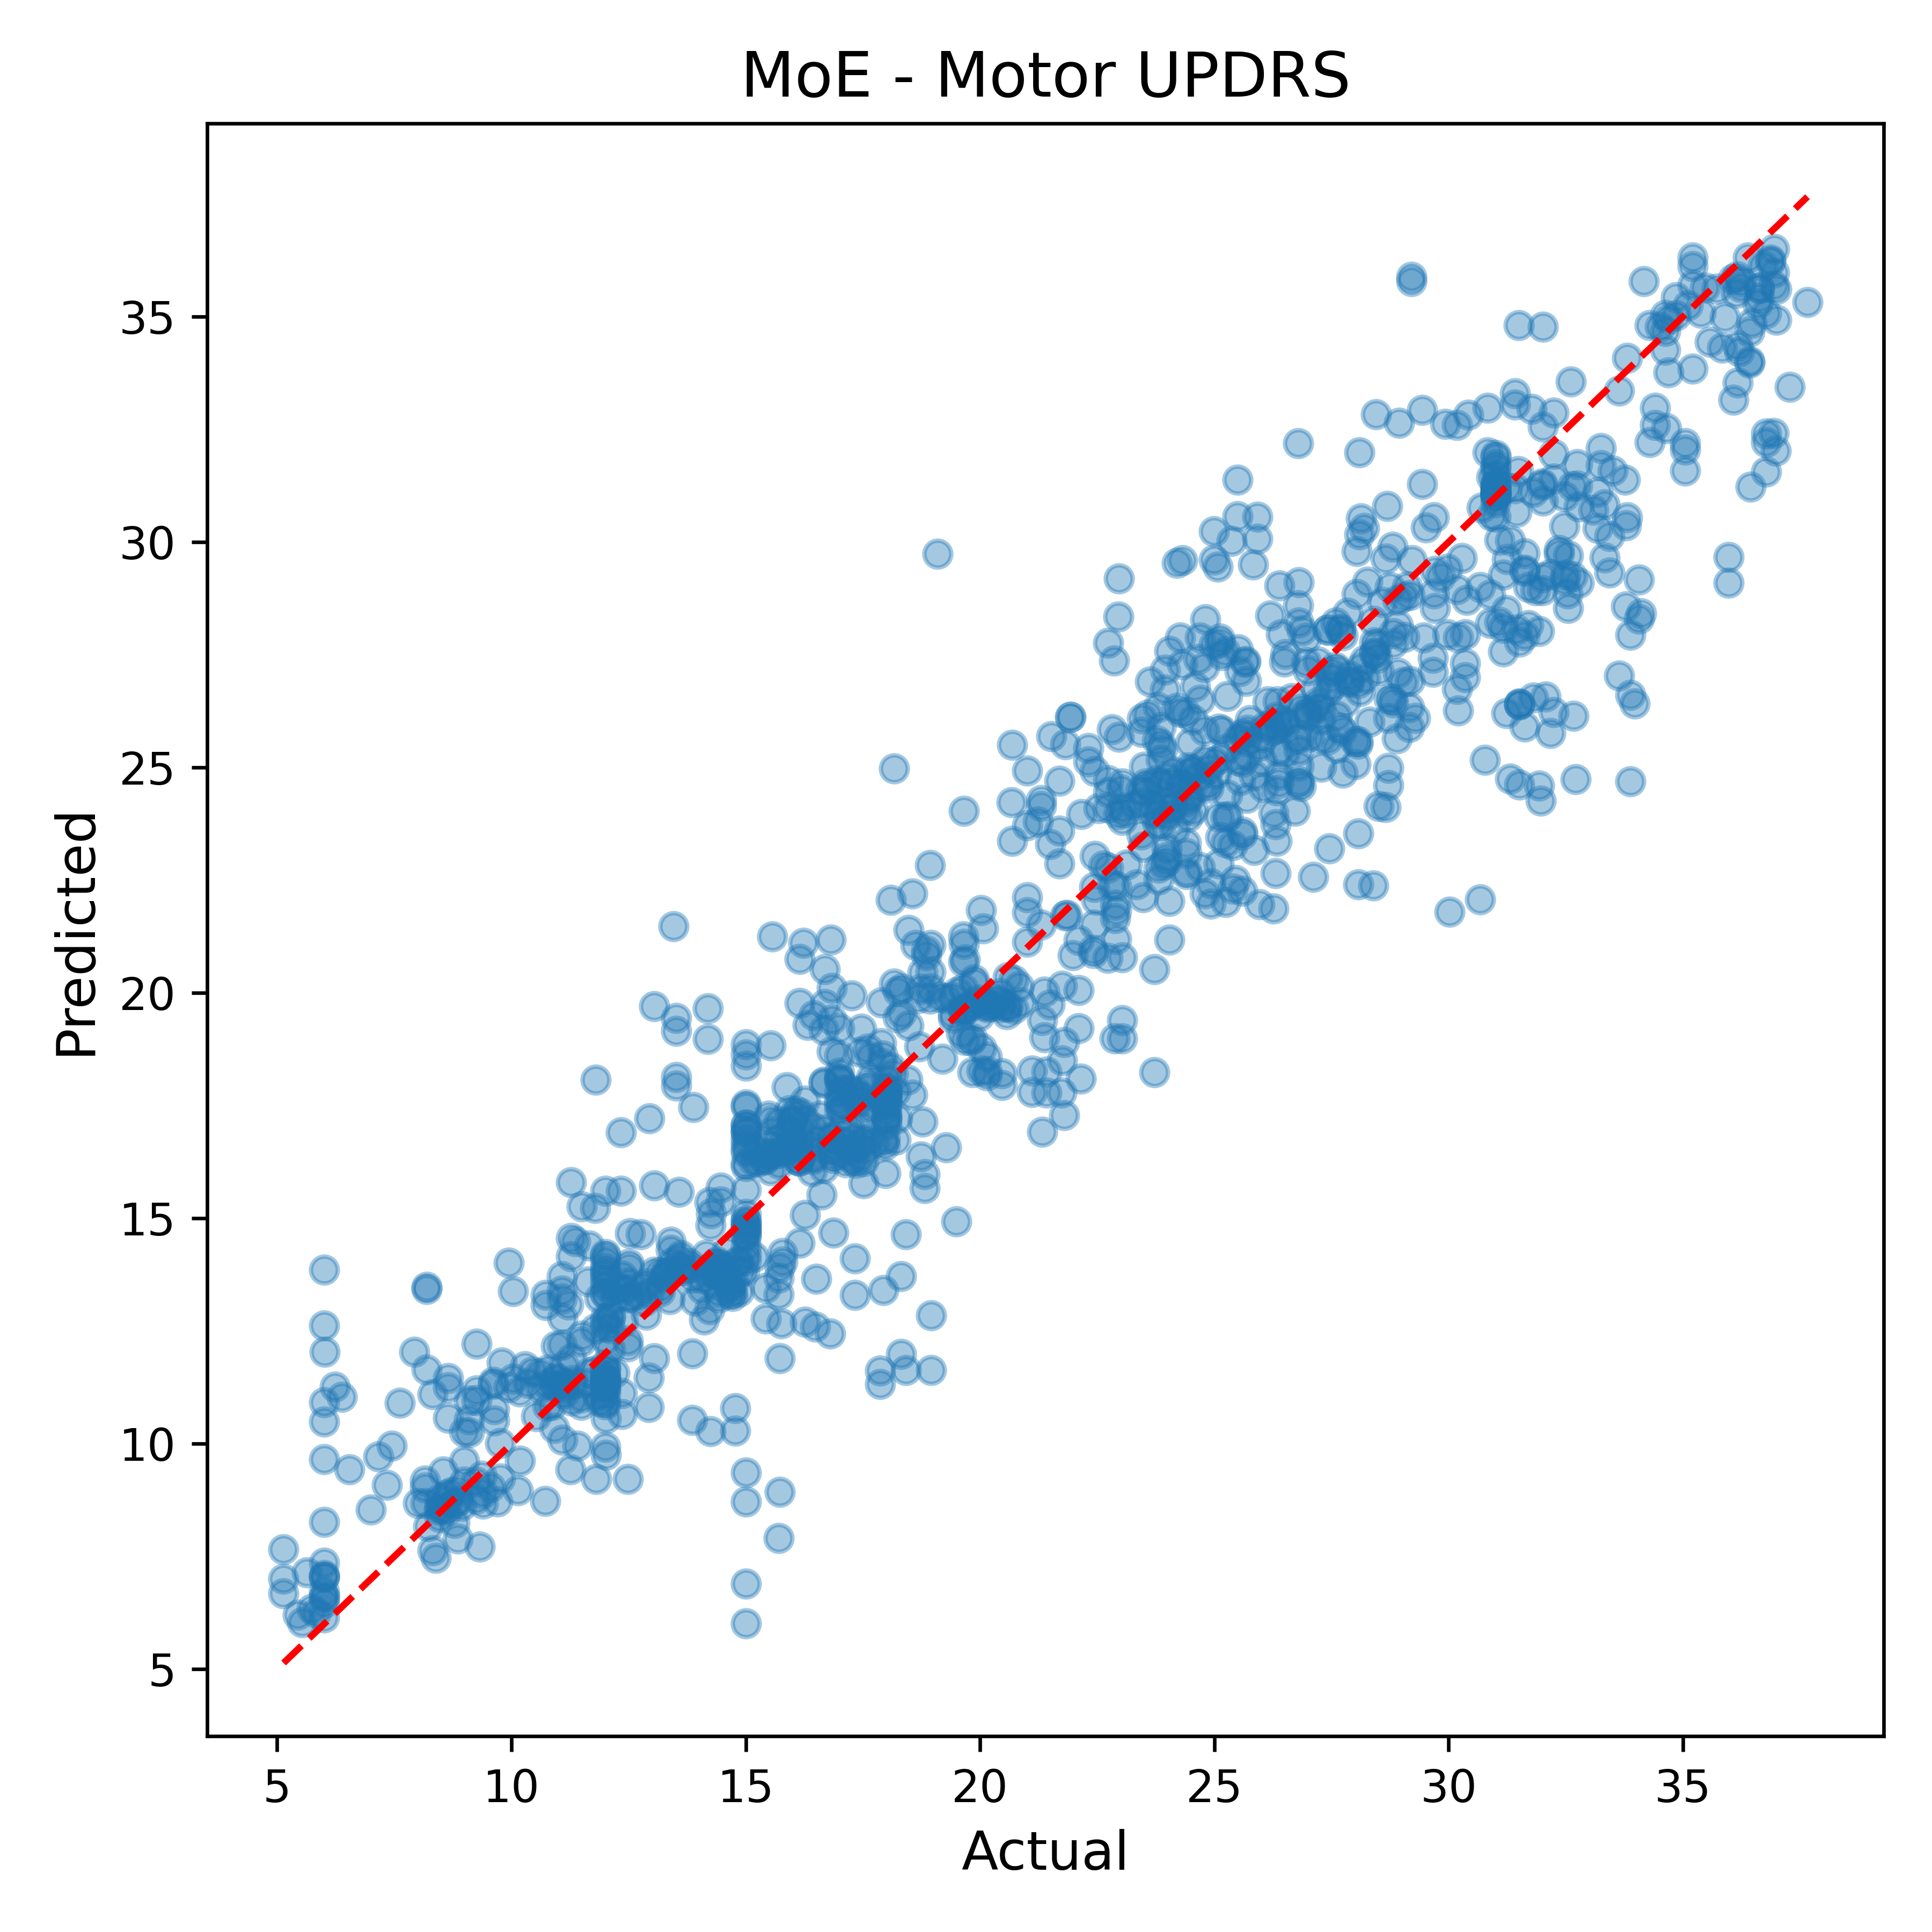
\includegraphics[width=\linewidth]{images/moe_-_motor_updrs_actual_vs_pred.png}
			\caption{MoE – Motor}
		\end{subfigure}
		\hfill
		\begin{subfigure}{0.45\linewidth}
			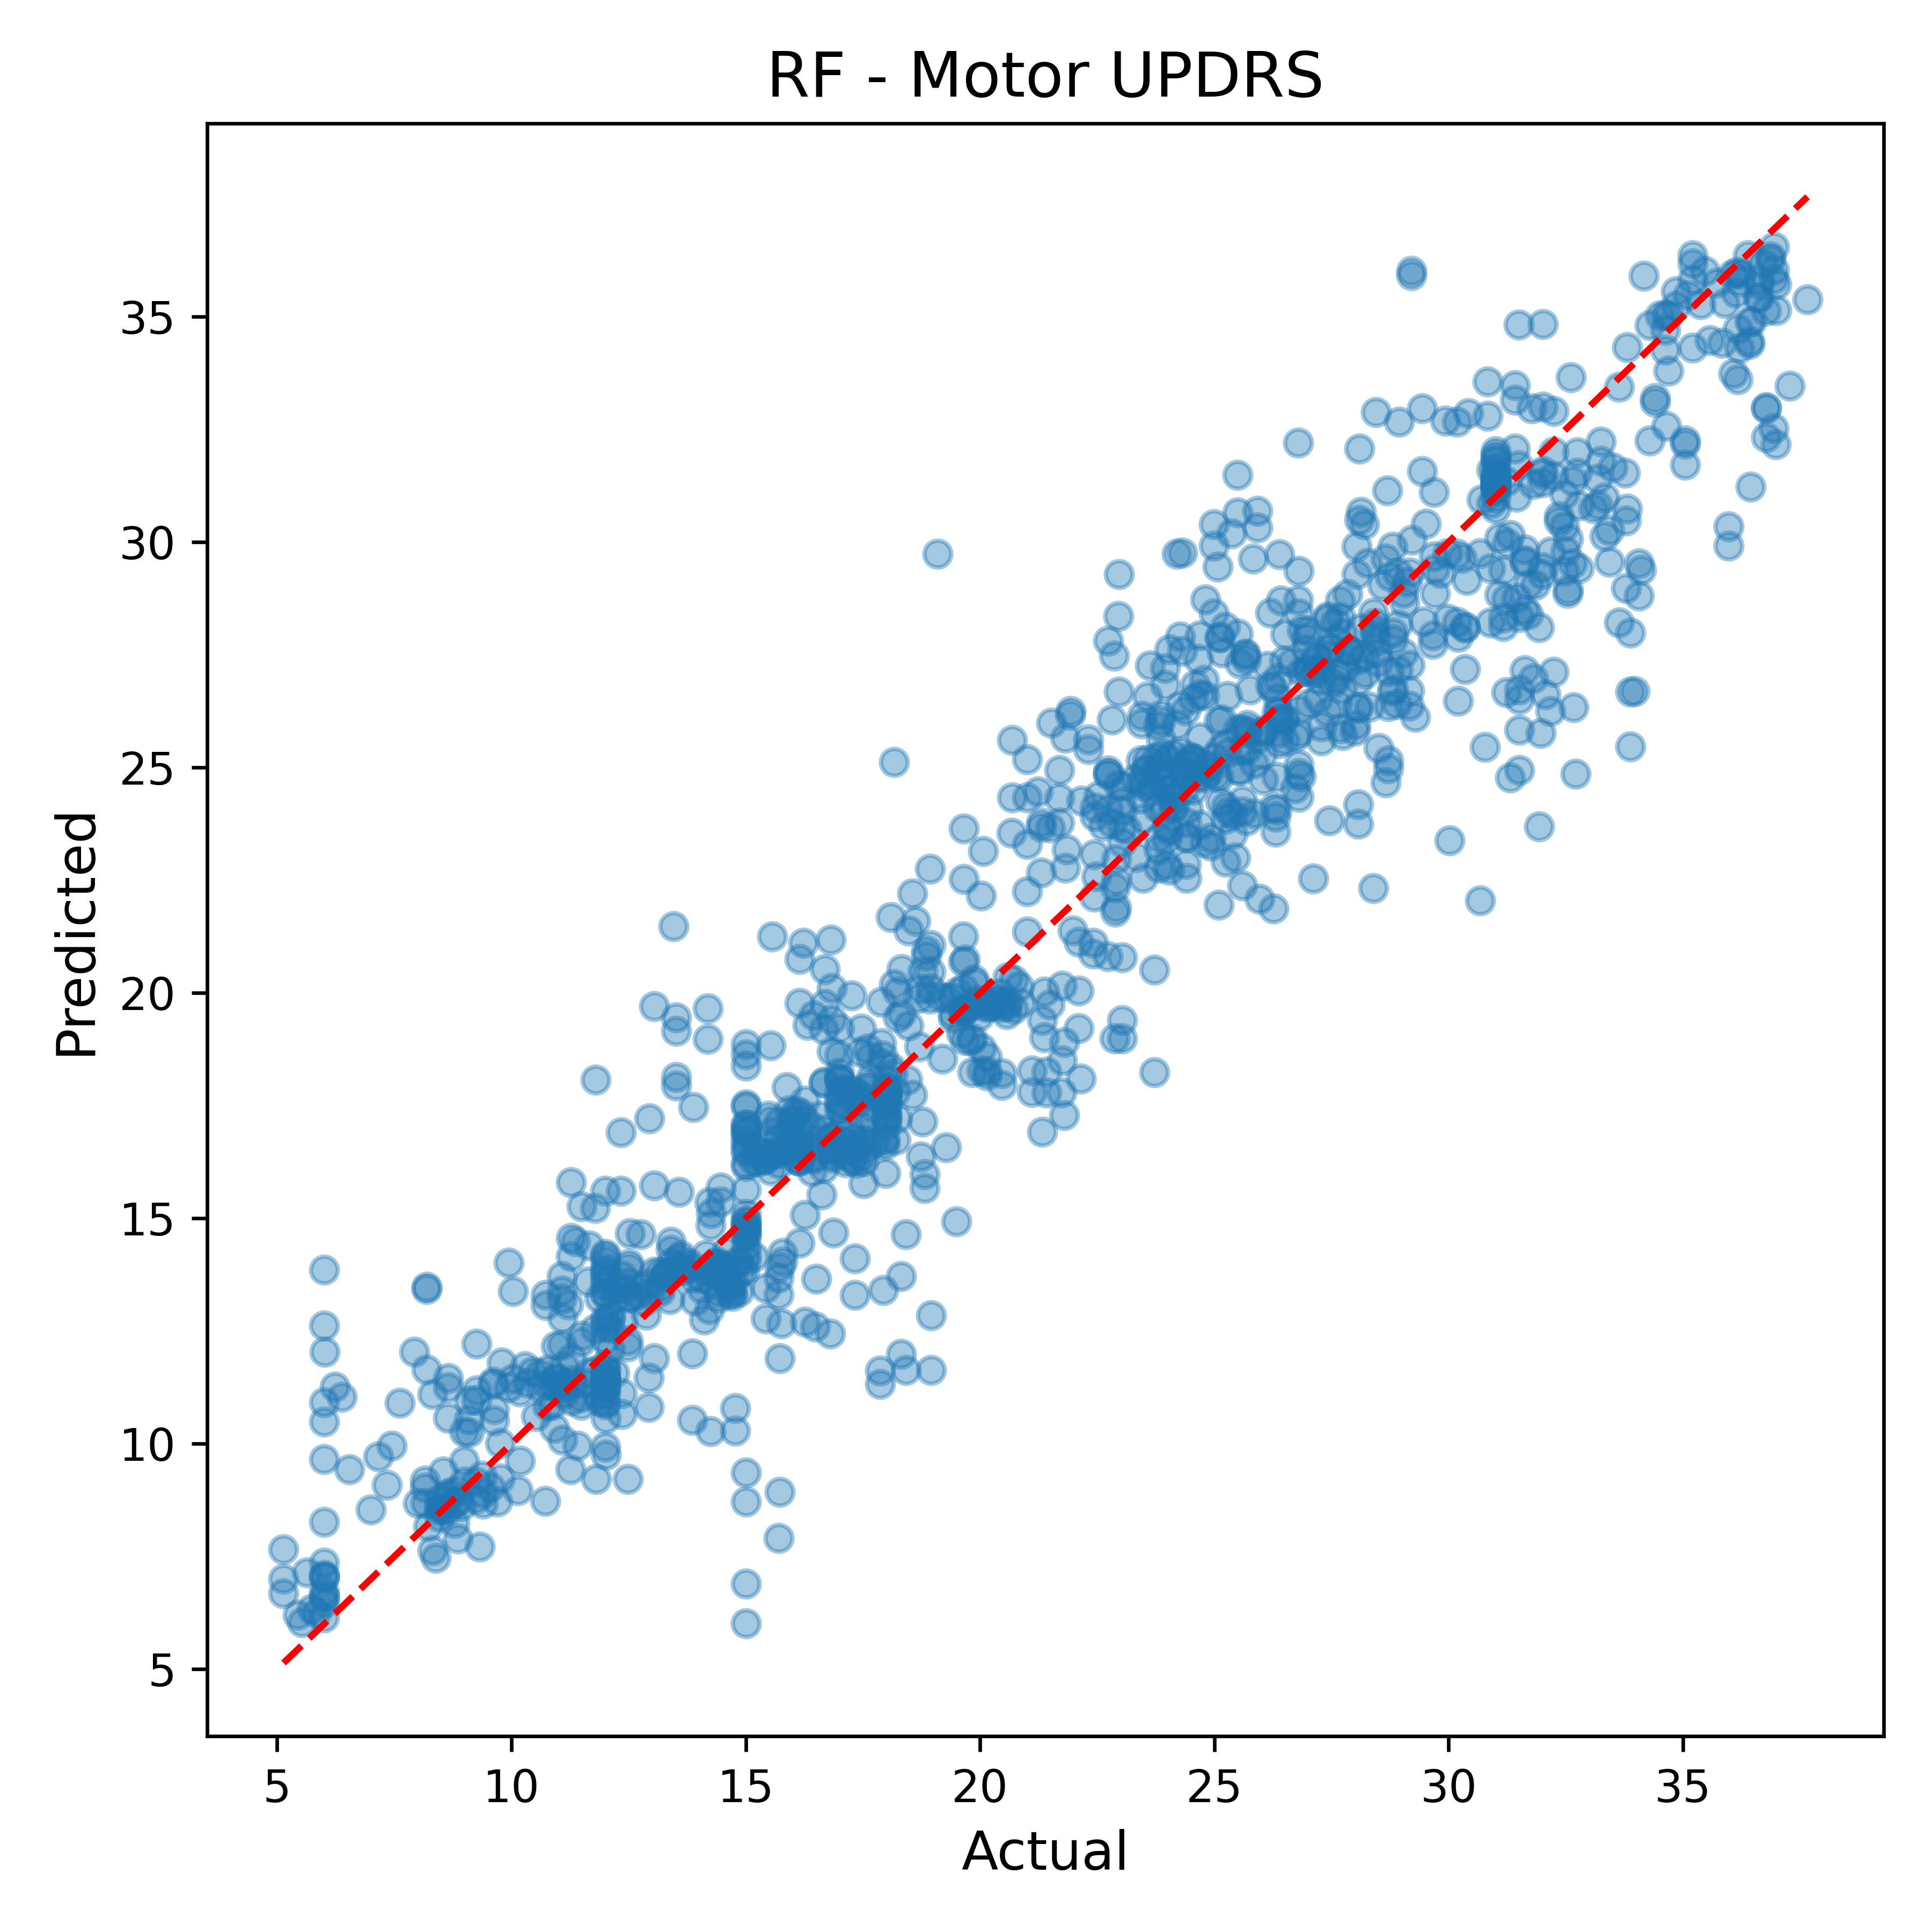
\includegraphics[width=\linewidth]{images/rf_-_motor_updrs_actual_vs_pred.png}
			\caption{Random Forest – Motor}
		\end{subfigure}
		
		\vspace{0.5cm}
		
		\begin{subfigure}{0.45\linewidth}
			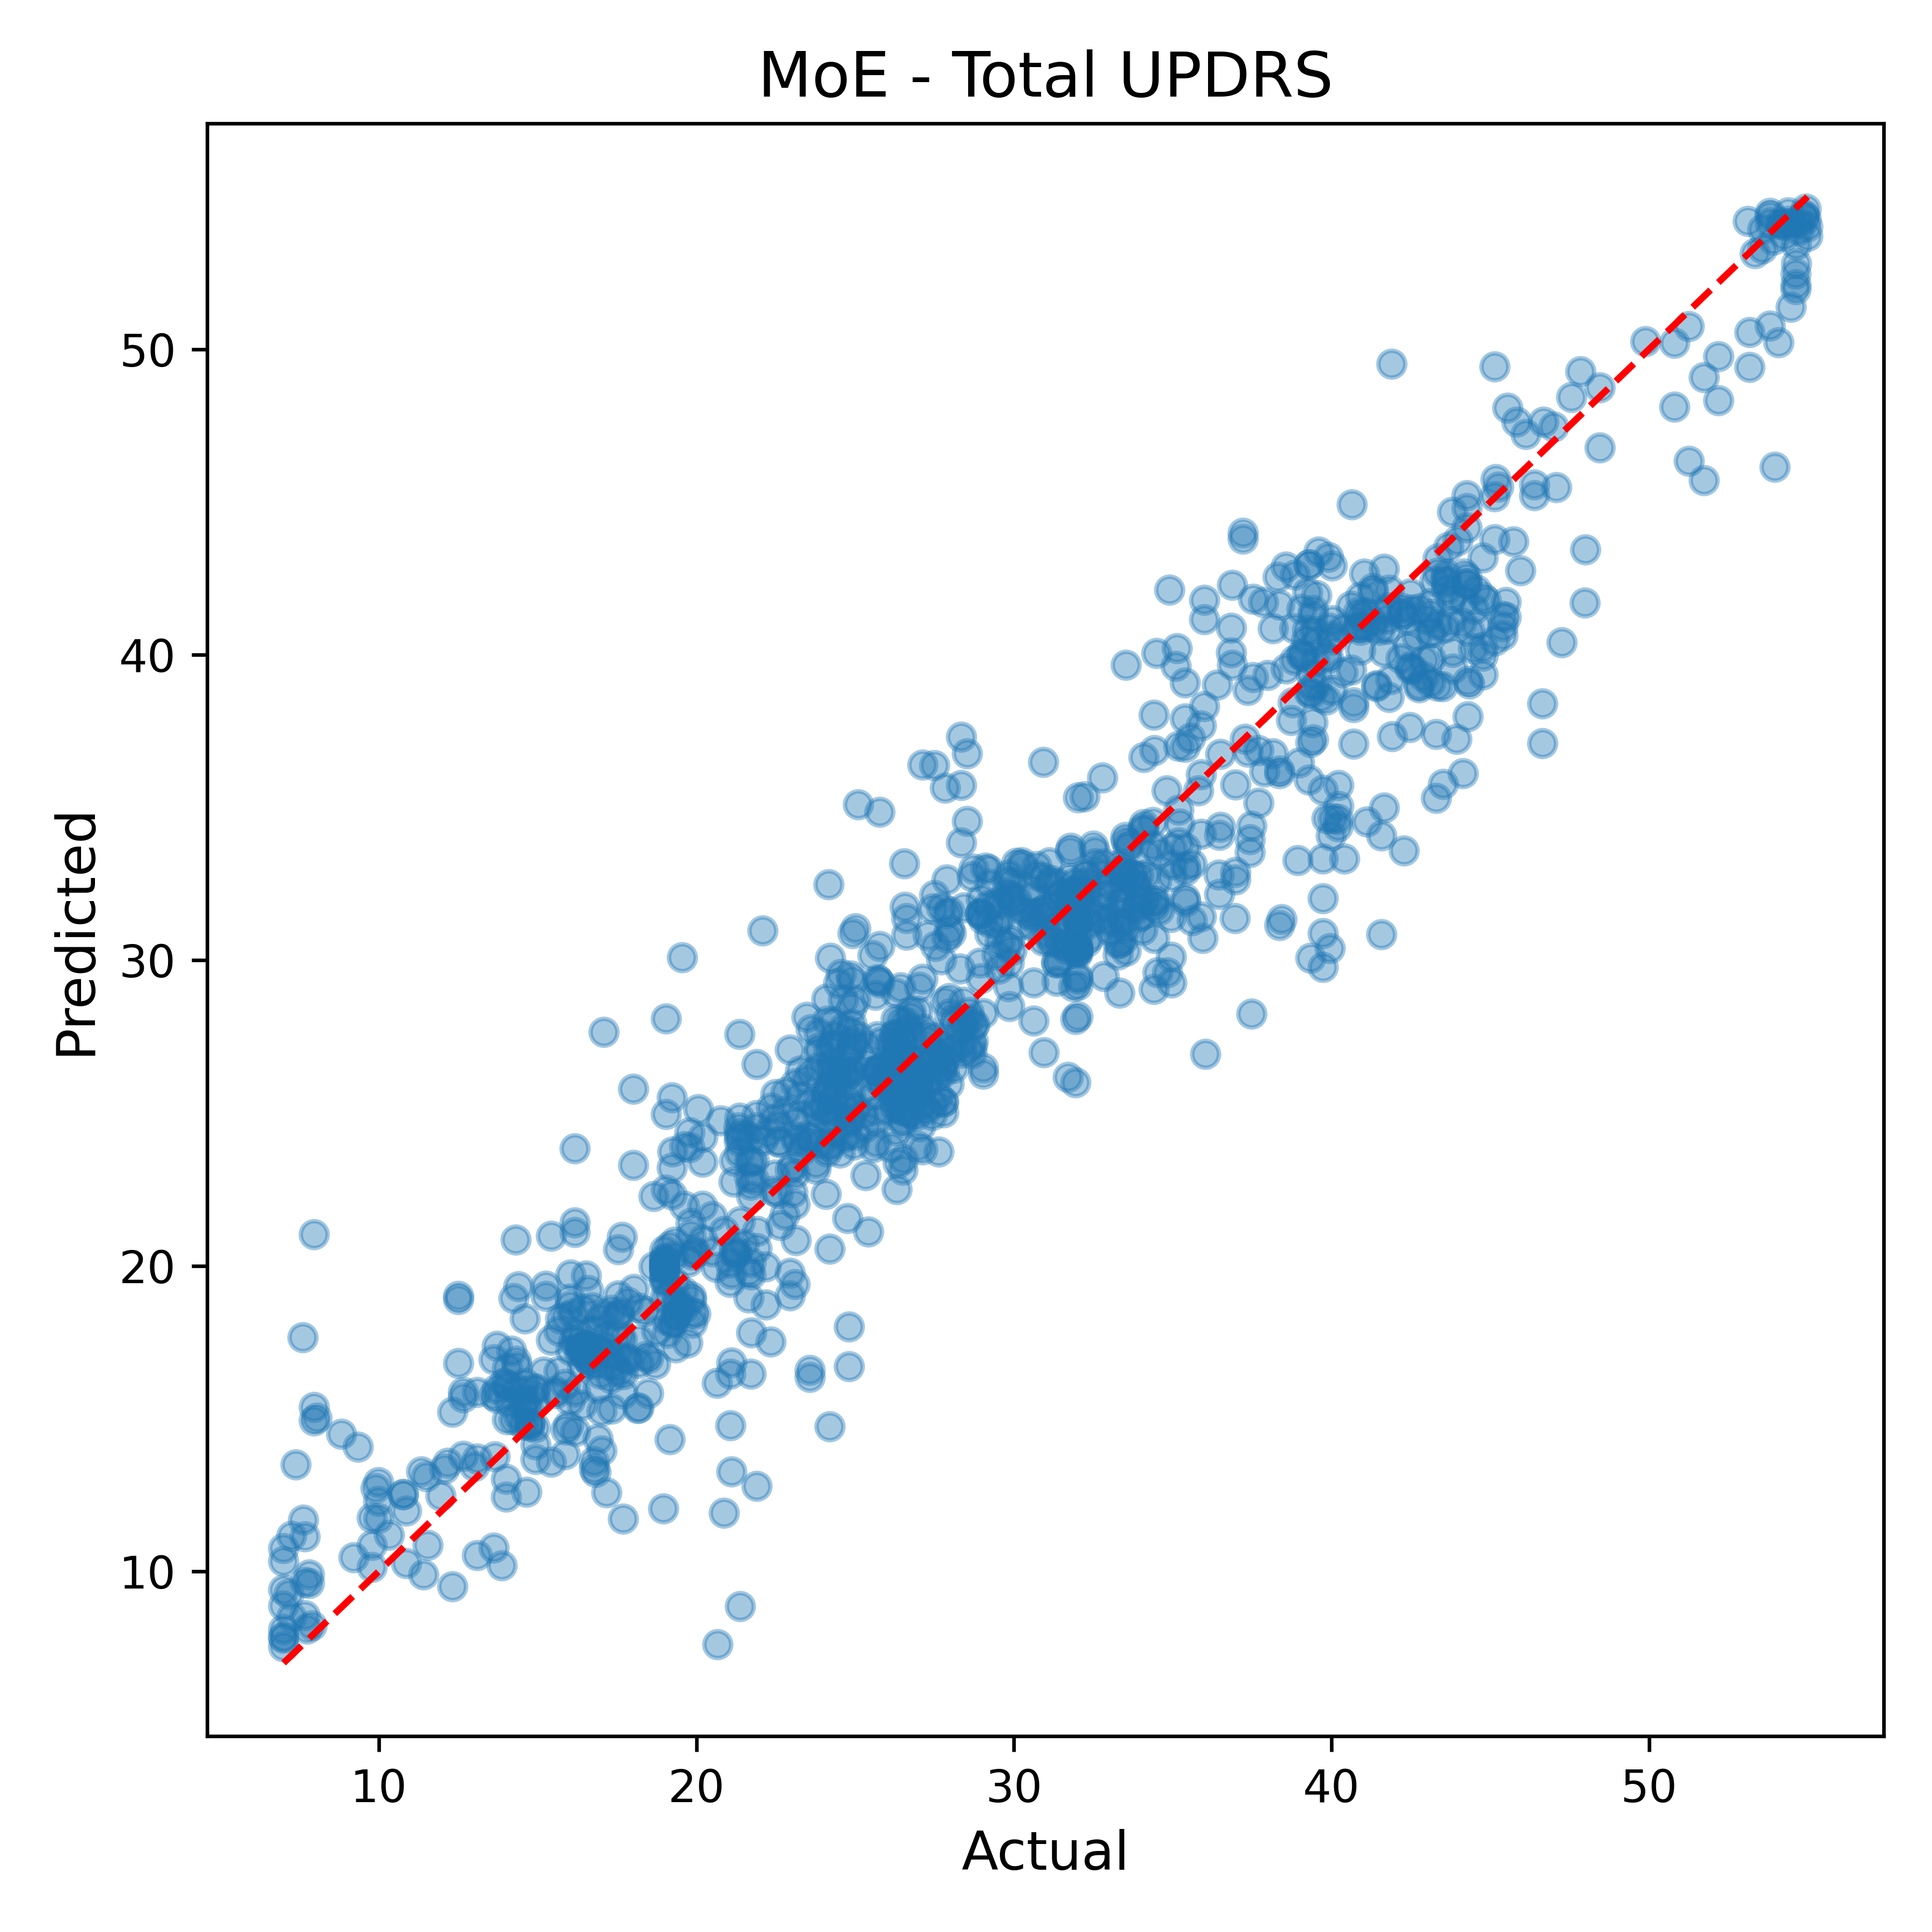
\includegraphics[width=\linewidth]{images/moe_-_total_updrs_actual_vs_pred.png}
			\caption{MoE – Total}
		\end{subfigure}
		\hfill
		\begin{subfigure}{0.45\linewidth}
			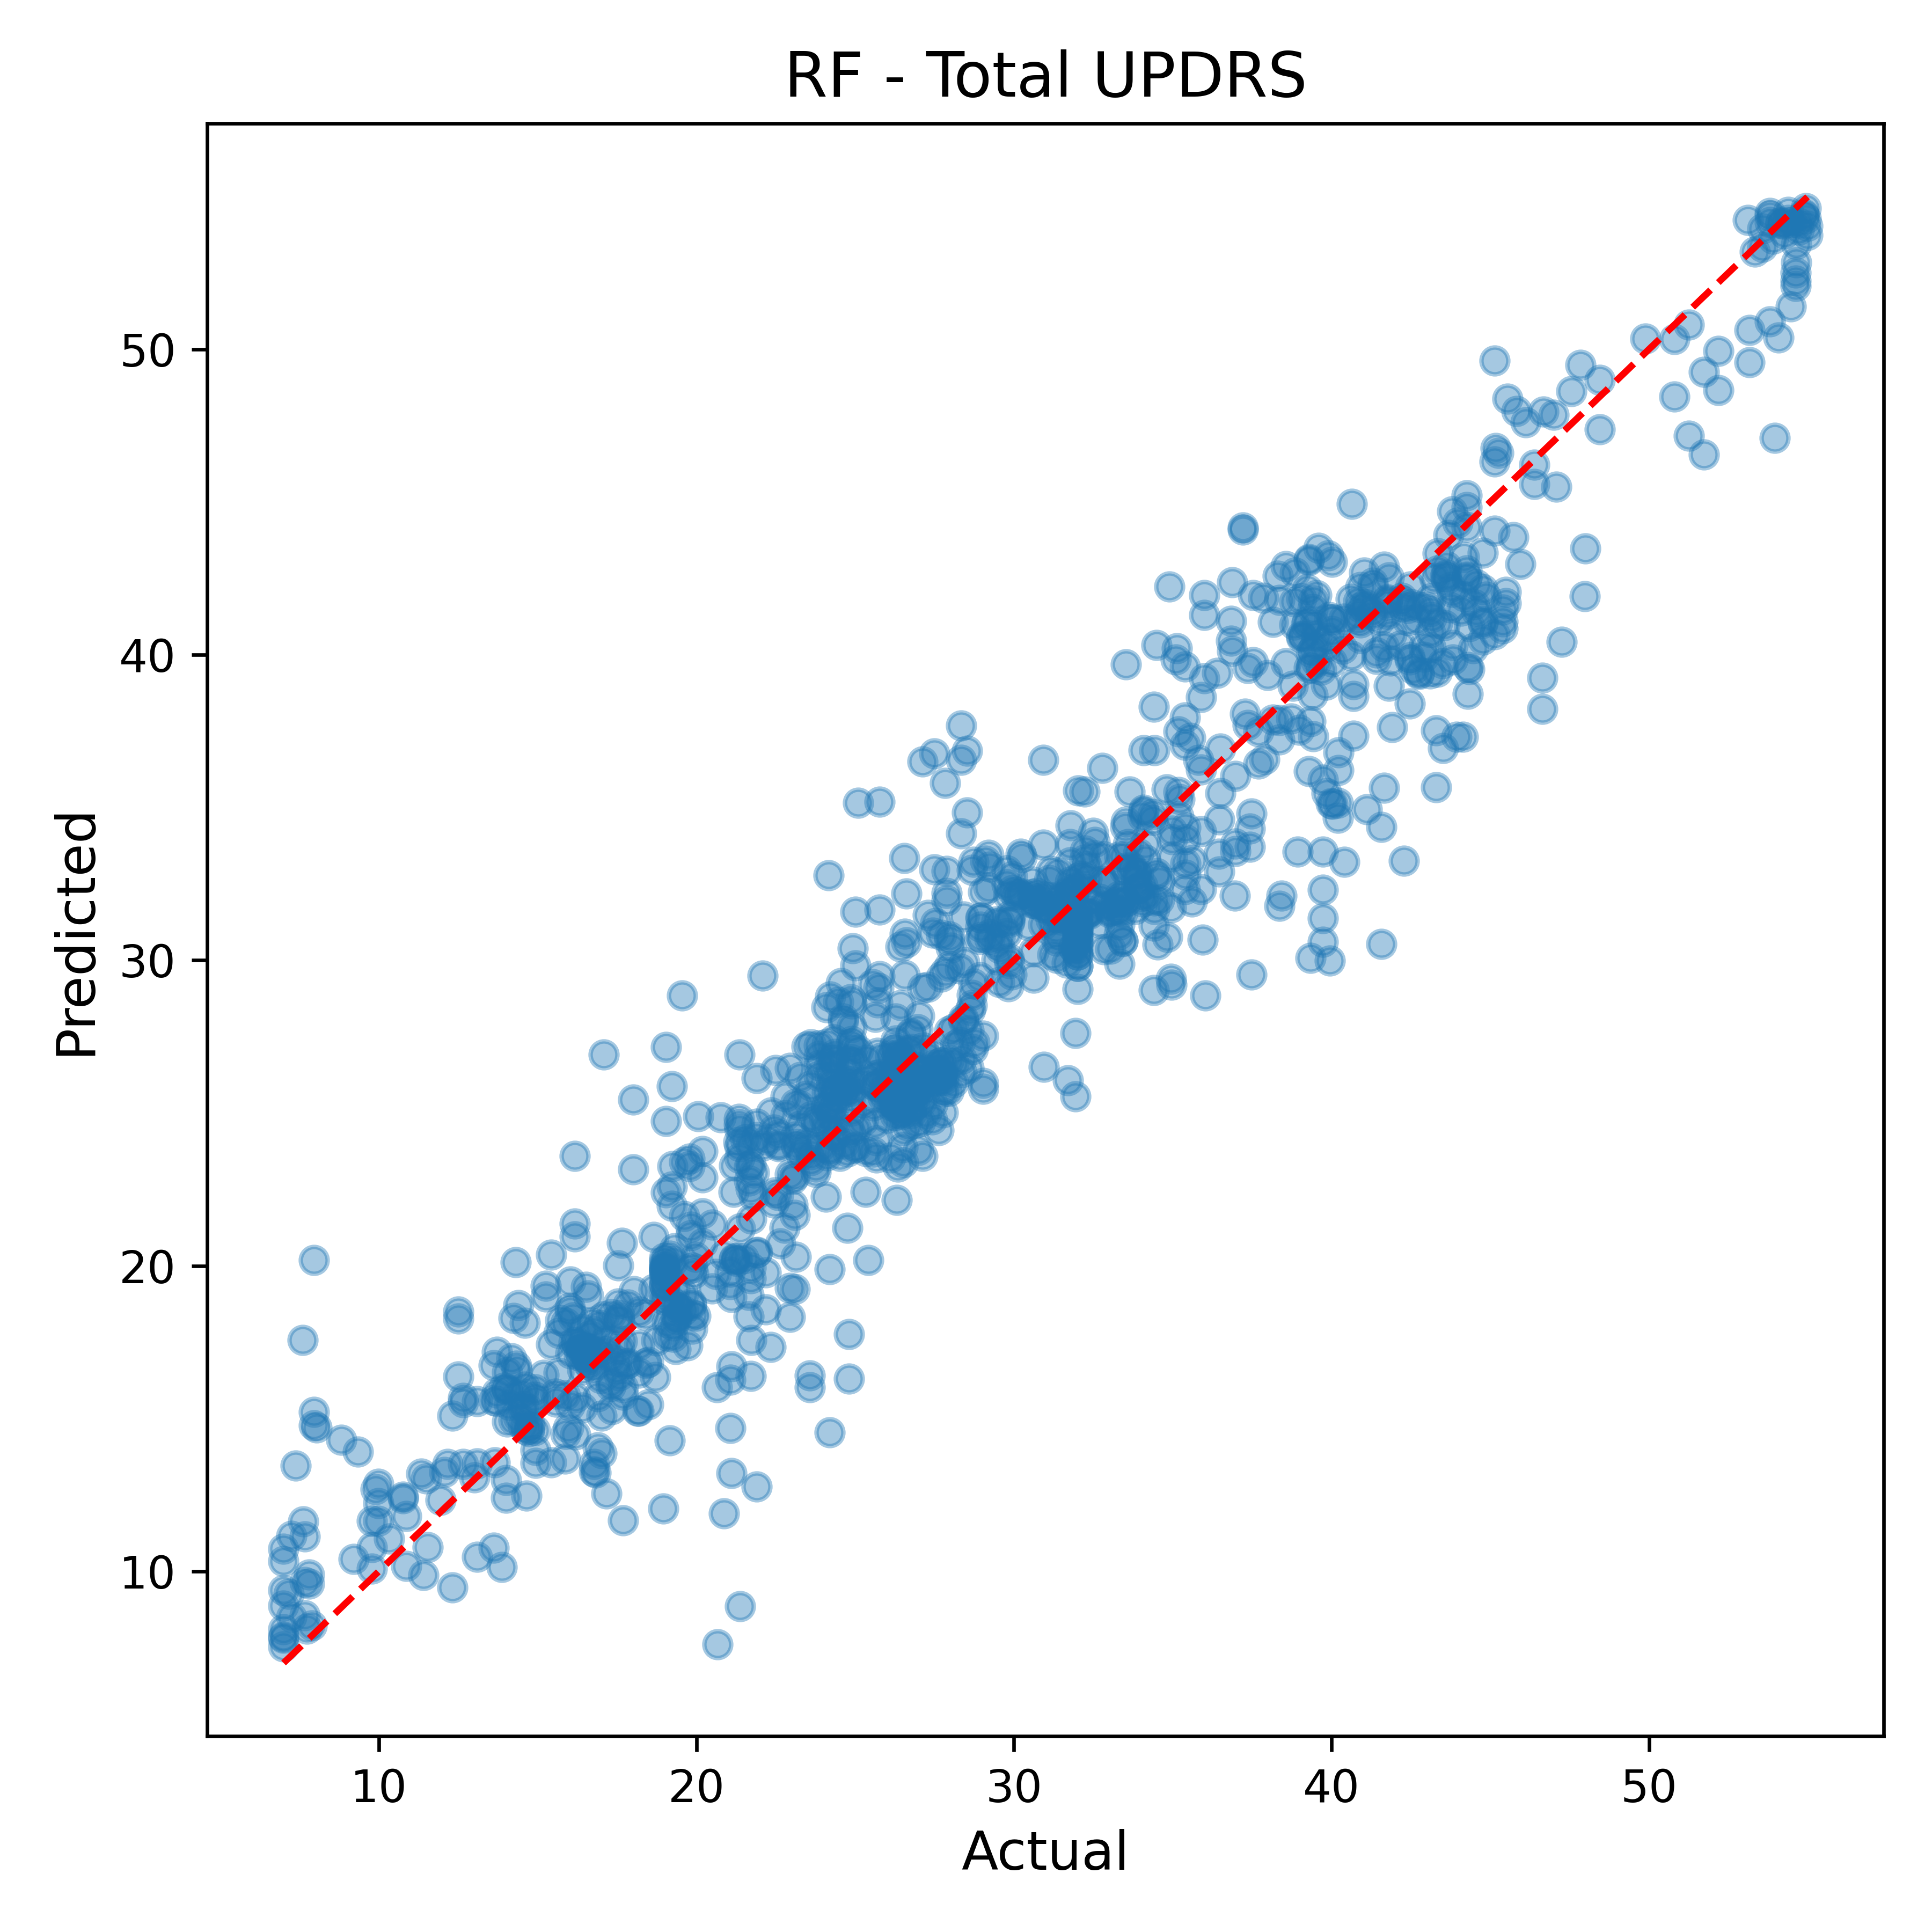
\includegraphics[width=\linewidth]{images/rf_-_total_updrs_actual_vs_pred.png}
			\caption{Random Forest – Total}
		\end{subfigure}
		
		\caption{Actual versus predicted severity scores for the MoE and Random Forest models. Both models demonstrate strong calibration across severity ranges, with Random Forest exhibiting slightly tighter dispersion around the identity line.}
		\label{fig:actual_vs_pred_main}
	\end{figure}
	
	\subsection{Residual Structure and Error Behavior}
	
	Although aggregate measures can be used to measure predictive accuracy, residual analysis offers better information regarding the bias and structure of error in the model. Residual patterns of the entropy-regularized Mixture of Experts in both $motor\_UPDRS$ and $total\_UPDRS$; and the overall prediction using the total predictor is shown in Figure \ref{fig:moe_residuals}. Ideally, the residual values are supposed to be concentrated around zero without any pattern of the severity range. The distributions in question are close to zero mean and have near-symmetric dispersion, which means that there is little systemic bias. Moreover, there is no noticeable heteroscedastic tendency which indicates that the variance in prediction does not change significantly with low and high severity rates. The lack of regular patterns in the residual justifies the appropriateness of nonlinear adaptive modeling to the measurement of the complex mapping of the features of acoustic perturbation and clinical measures of severity.
	
	
	\begin{figure}[H]
		\centering
		\begin{subfigure}{0.45\linewidth}
			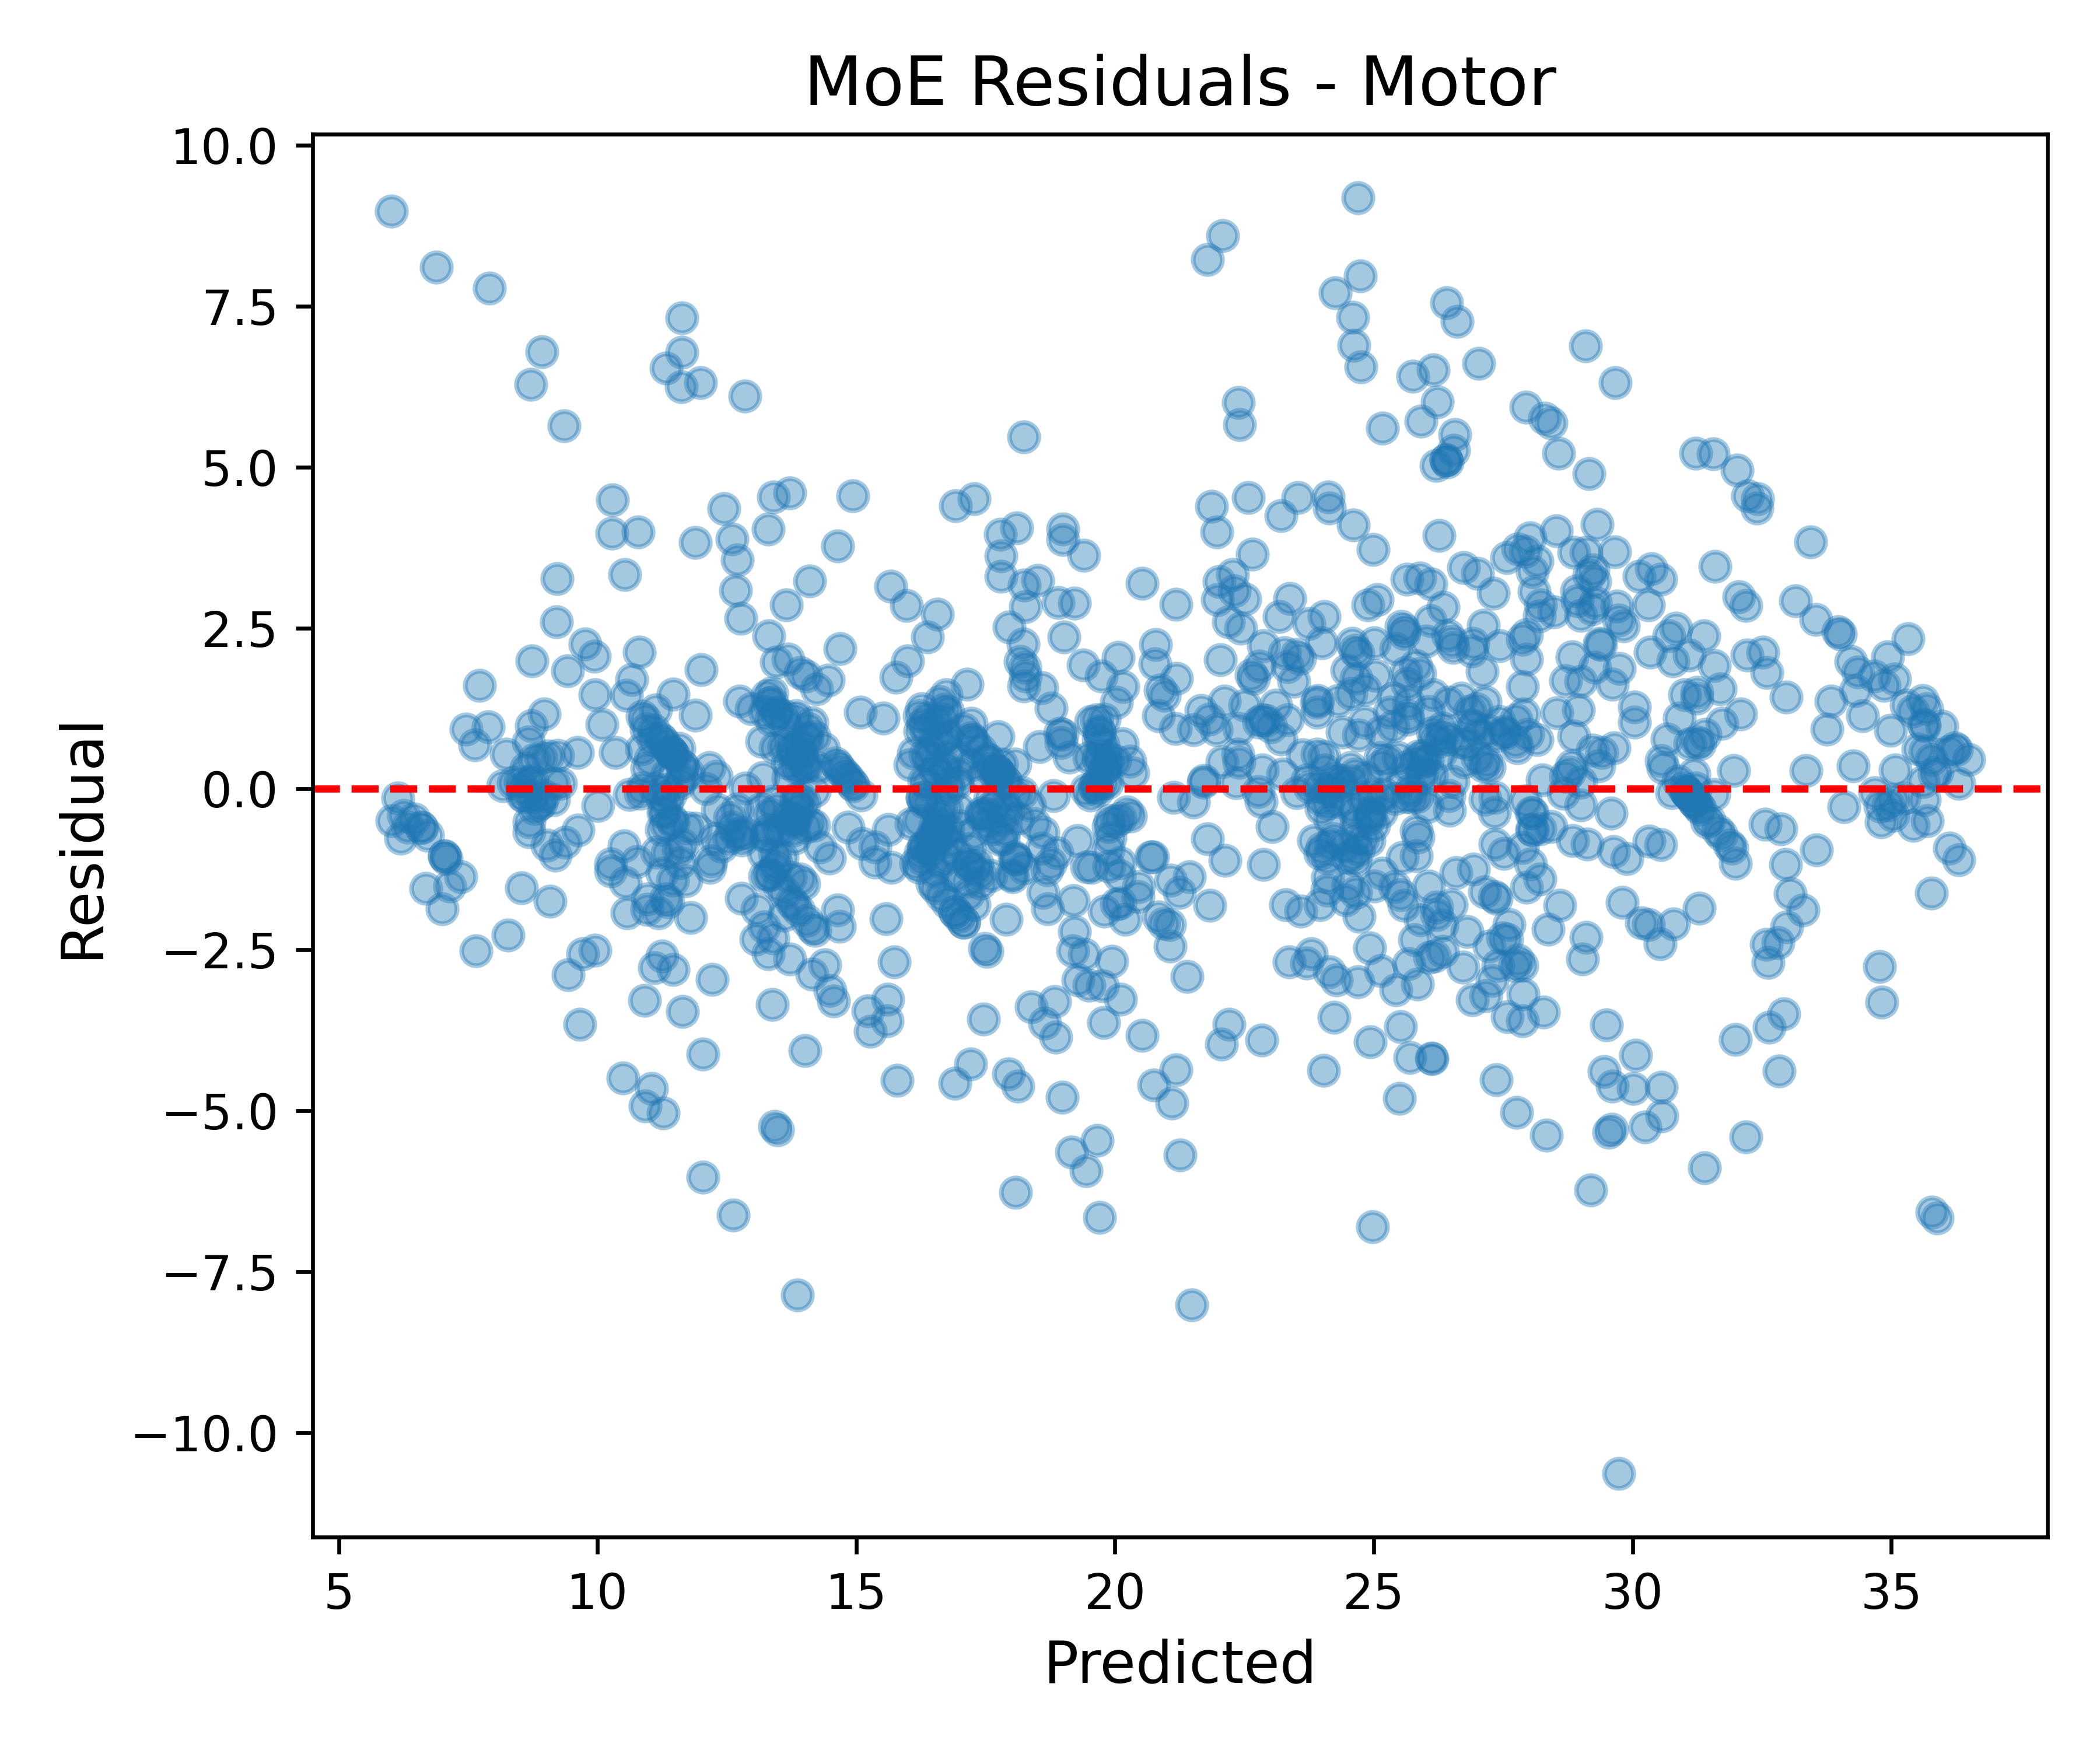
\includegraphics[width=\linewidth]{images/moe_residuals_-_motor_residuals.png}
			\caption{Motor Residuals}
		\end{subfigure}
		\hfill
		\begin{subfigure}{0.45\linewidth}
			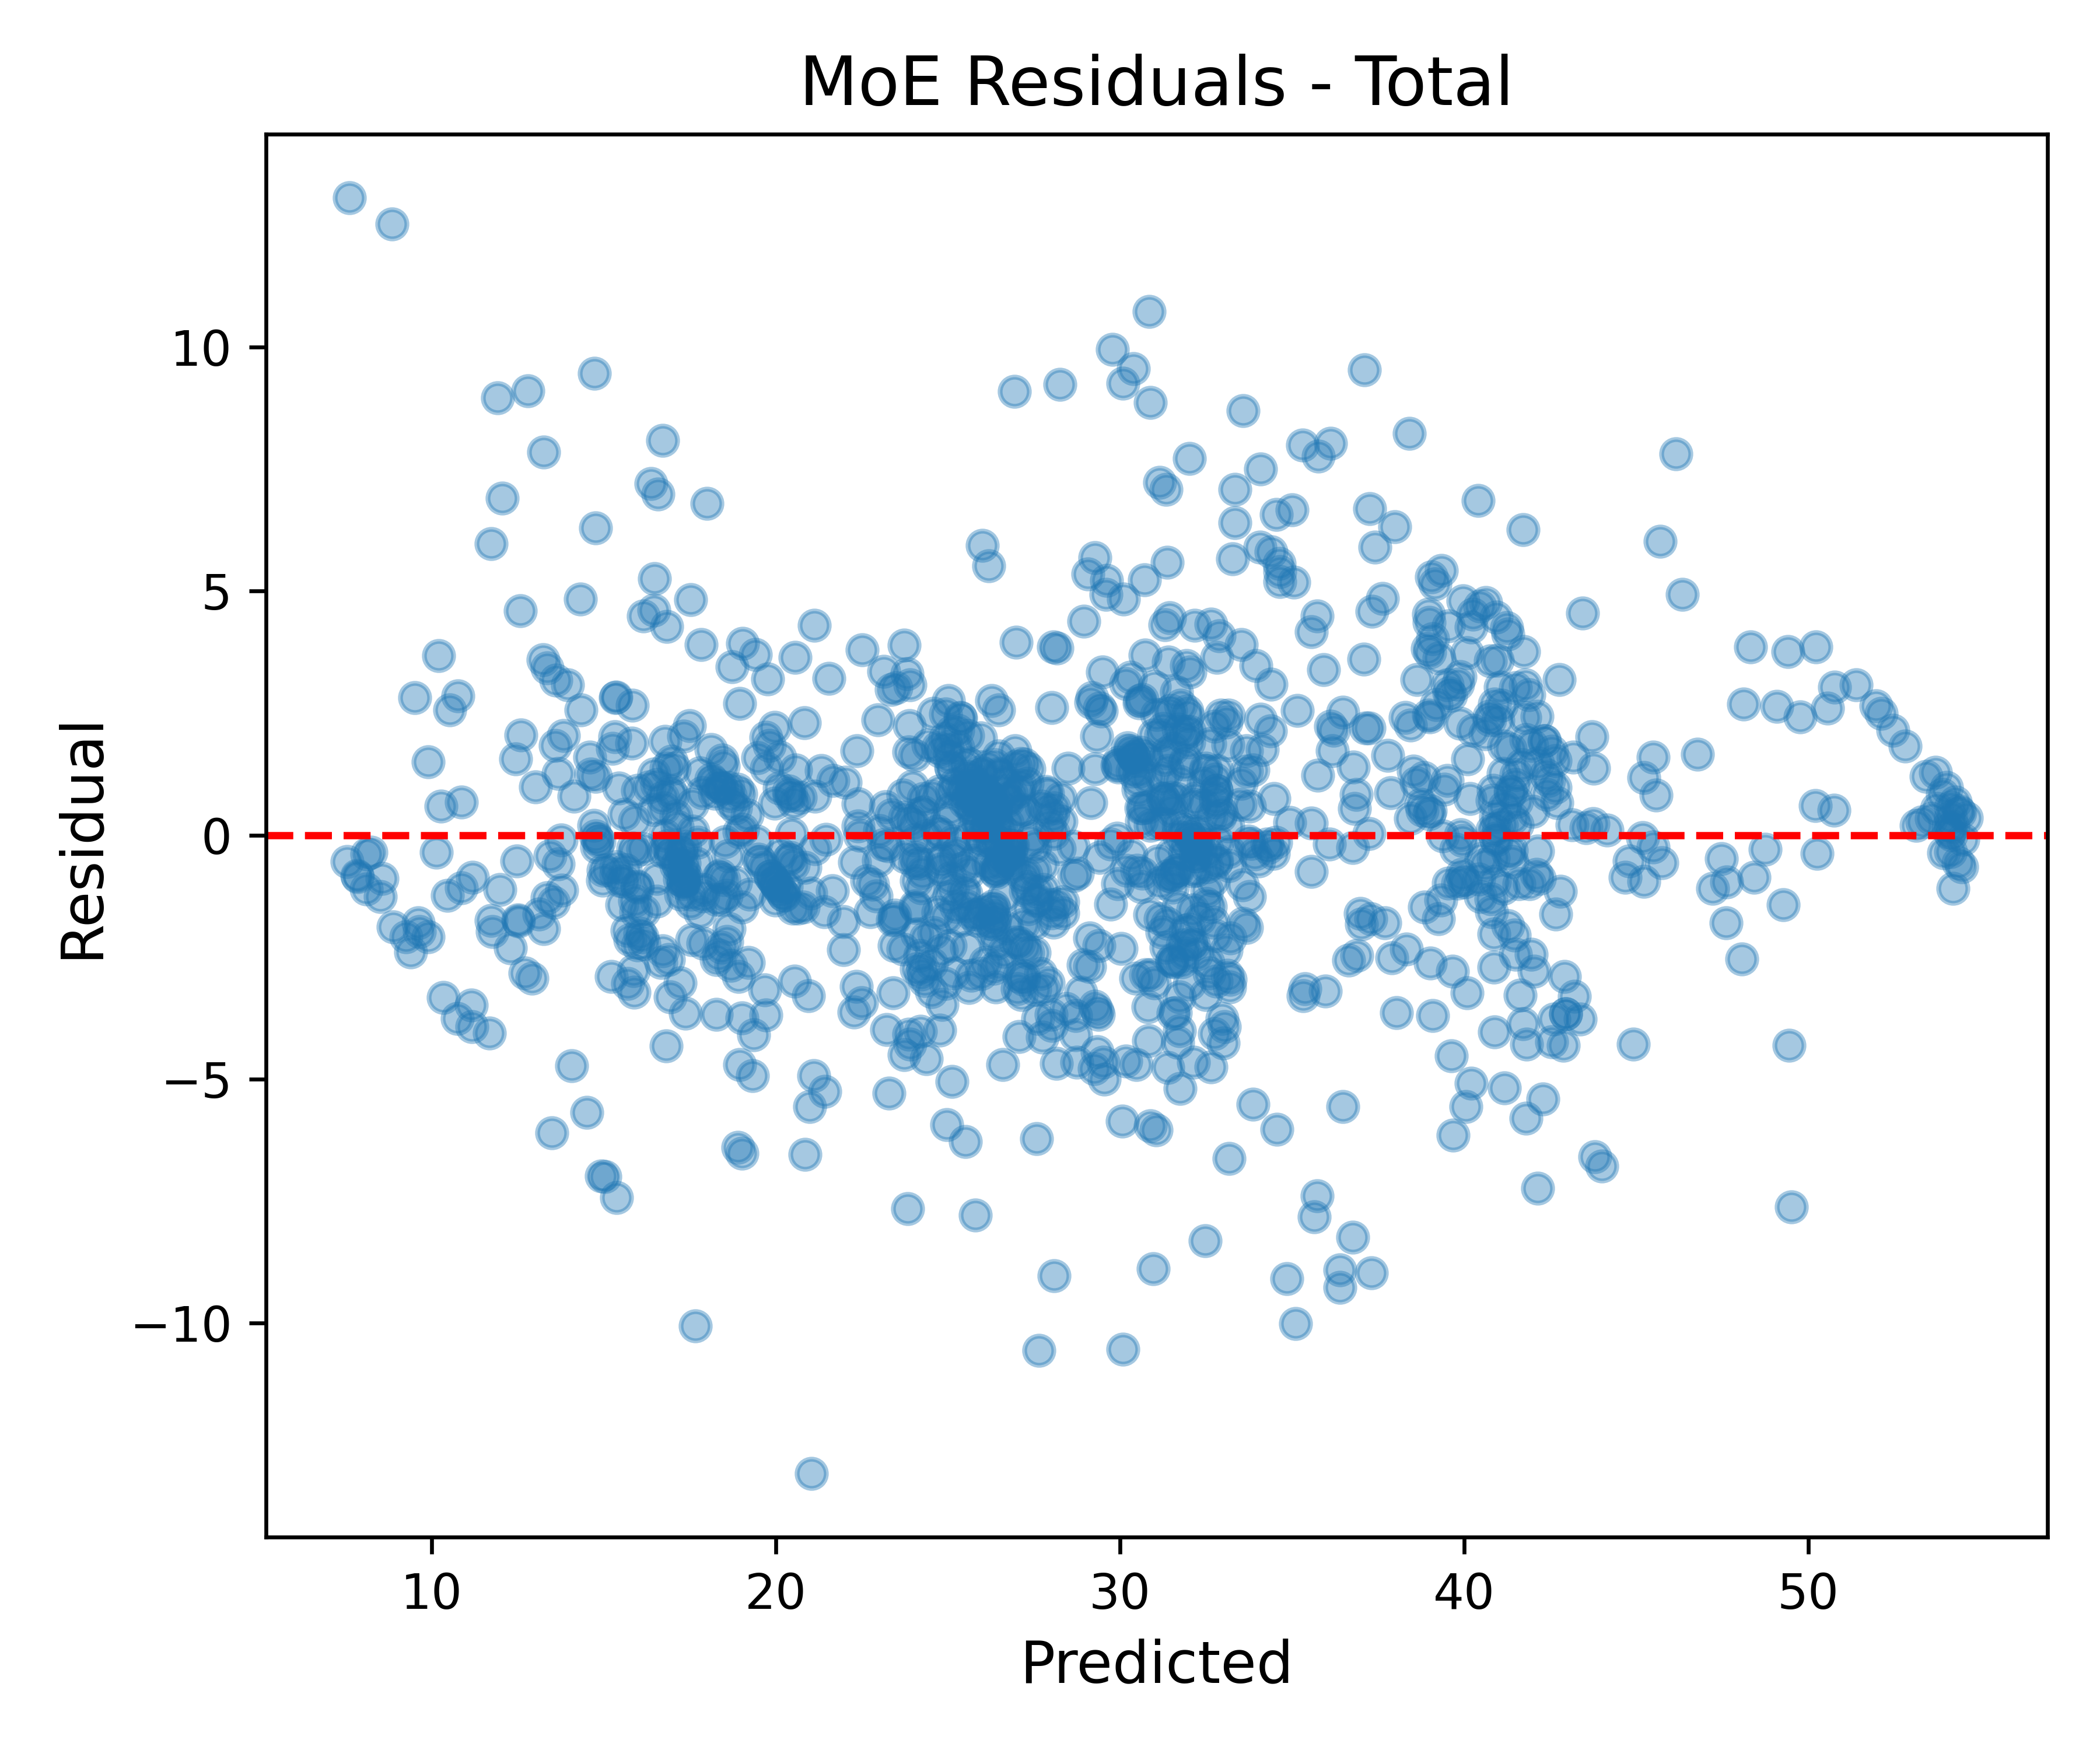
\includegraphics[width=\linewidth]{images/moe_residuals_-_total_residuals.png}
			\caption{Total Residuals}
		\end{subfigure}
		
		\caption{Residual analysis for the proposed entropy-regularized MoE. Residuals are centered around zero with approximately symmetric dispersion, indicating minimal systematic bias.}
		\label{fig:moe_residuals}
	\end{figure}
	\subsection{Adaptive Expert Weight Analysis}
	
	In addition to predictive accuracy, one of the aims of the proposed framework is to facilitate adaptive and target specialization of experts. The learned weight distributions of the expert weights in case of entropy regularization with both predictions, which are $motor\_UPDRS$ and $total\_UPDRS$ are shown in Figure \ref{fig:expert_weights}. The gating mechanism attributes convex weights on each expert on a sample-by-sample basis. Dissection of the acquired distributions shows the evident predominance of the Random Forest expert especially when severity of motor is estimated. The average motor weight of the Random Forest is greater than 0.92 which shows that tree-based nonlinear modeling takes into account most of the predictive structure in the acoustic-motor mapping. In the case of total severity prediction, the Random Forest is still dominant but has a slightly lower average weight (about 0.88) and greater input of the secondary experts. It implies that total severity incorporates more extensive signal properties which can develop complementary modeling properties. Notably, with the entropy regularization, there is no single authority that can collapse to a single expert and, thus, the goal of the mechanisms is to keep the contributions distributed and preserve the adaptive potential of the ensemble. These results show that the offered MoE framework does not only attain the competitive performance level but also offers an interpretable view of the expert specialization across clinical targets.
	\begin{figure}[H]
		\centering
		\begin{subfigure}{0.6\linewidth}
			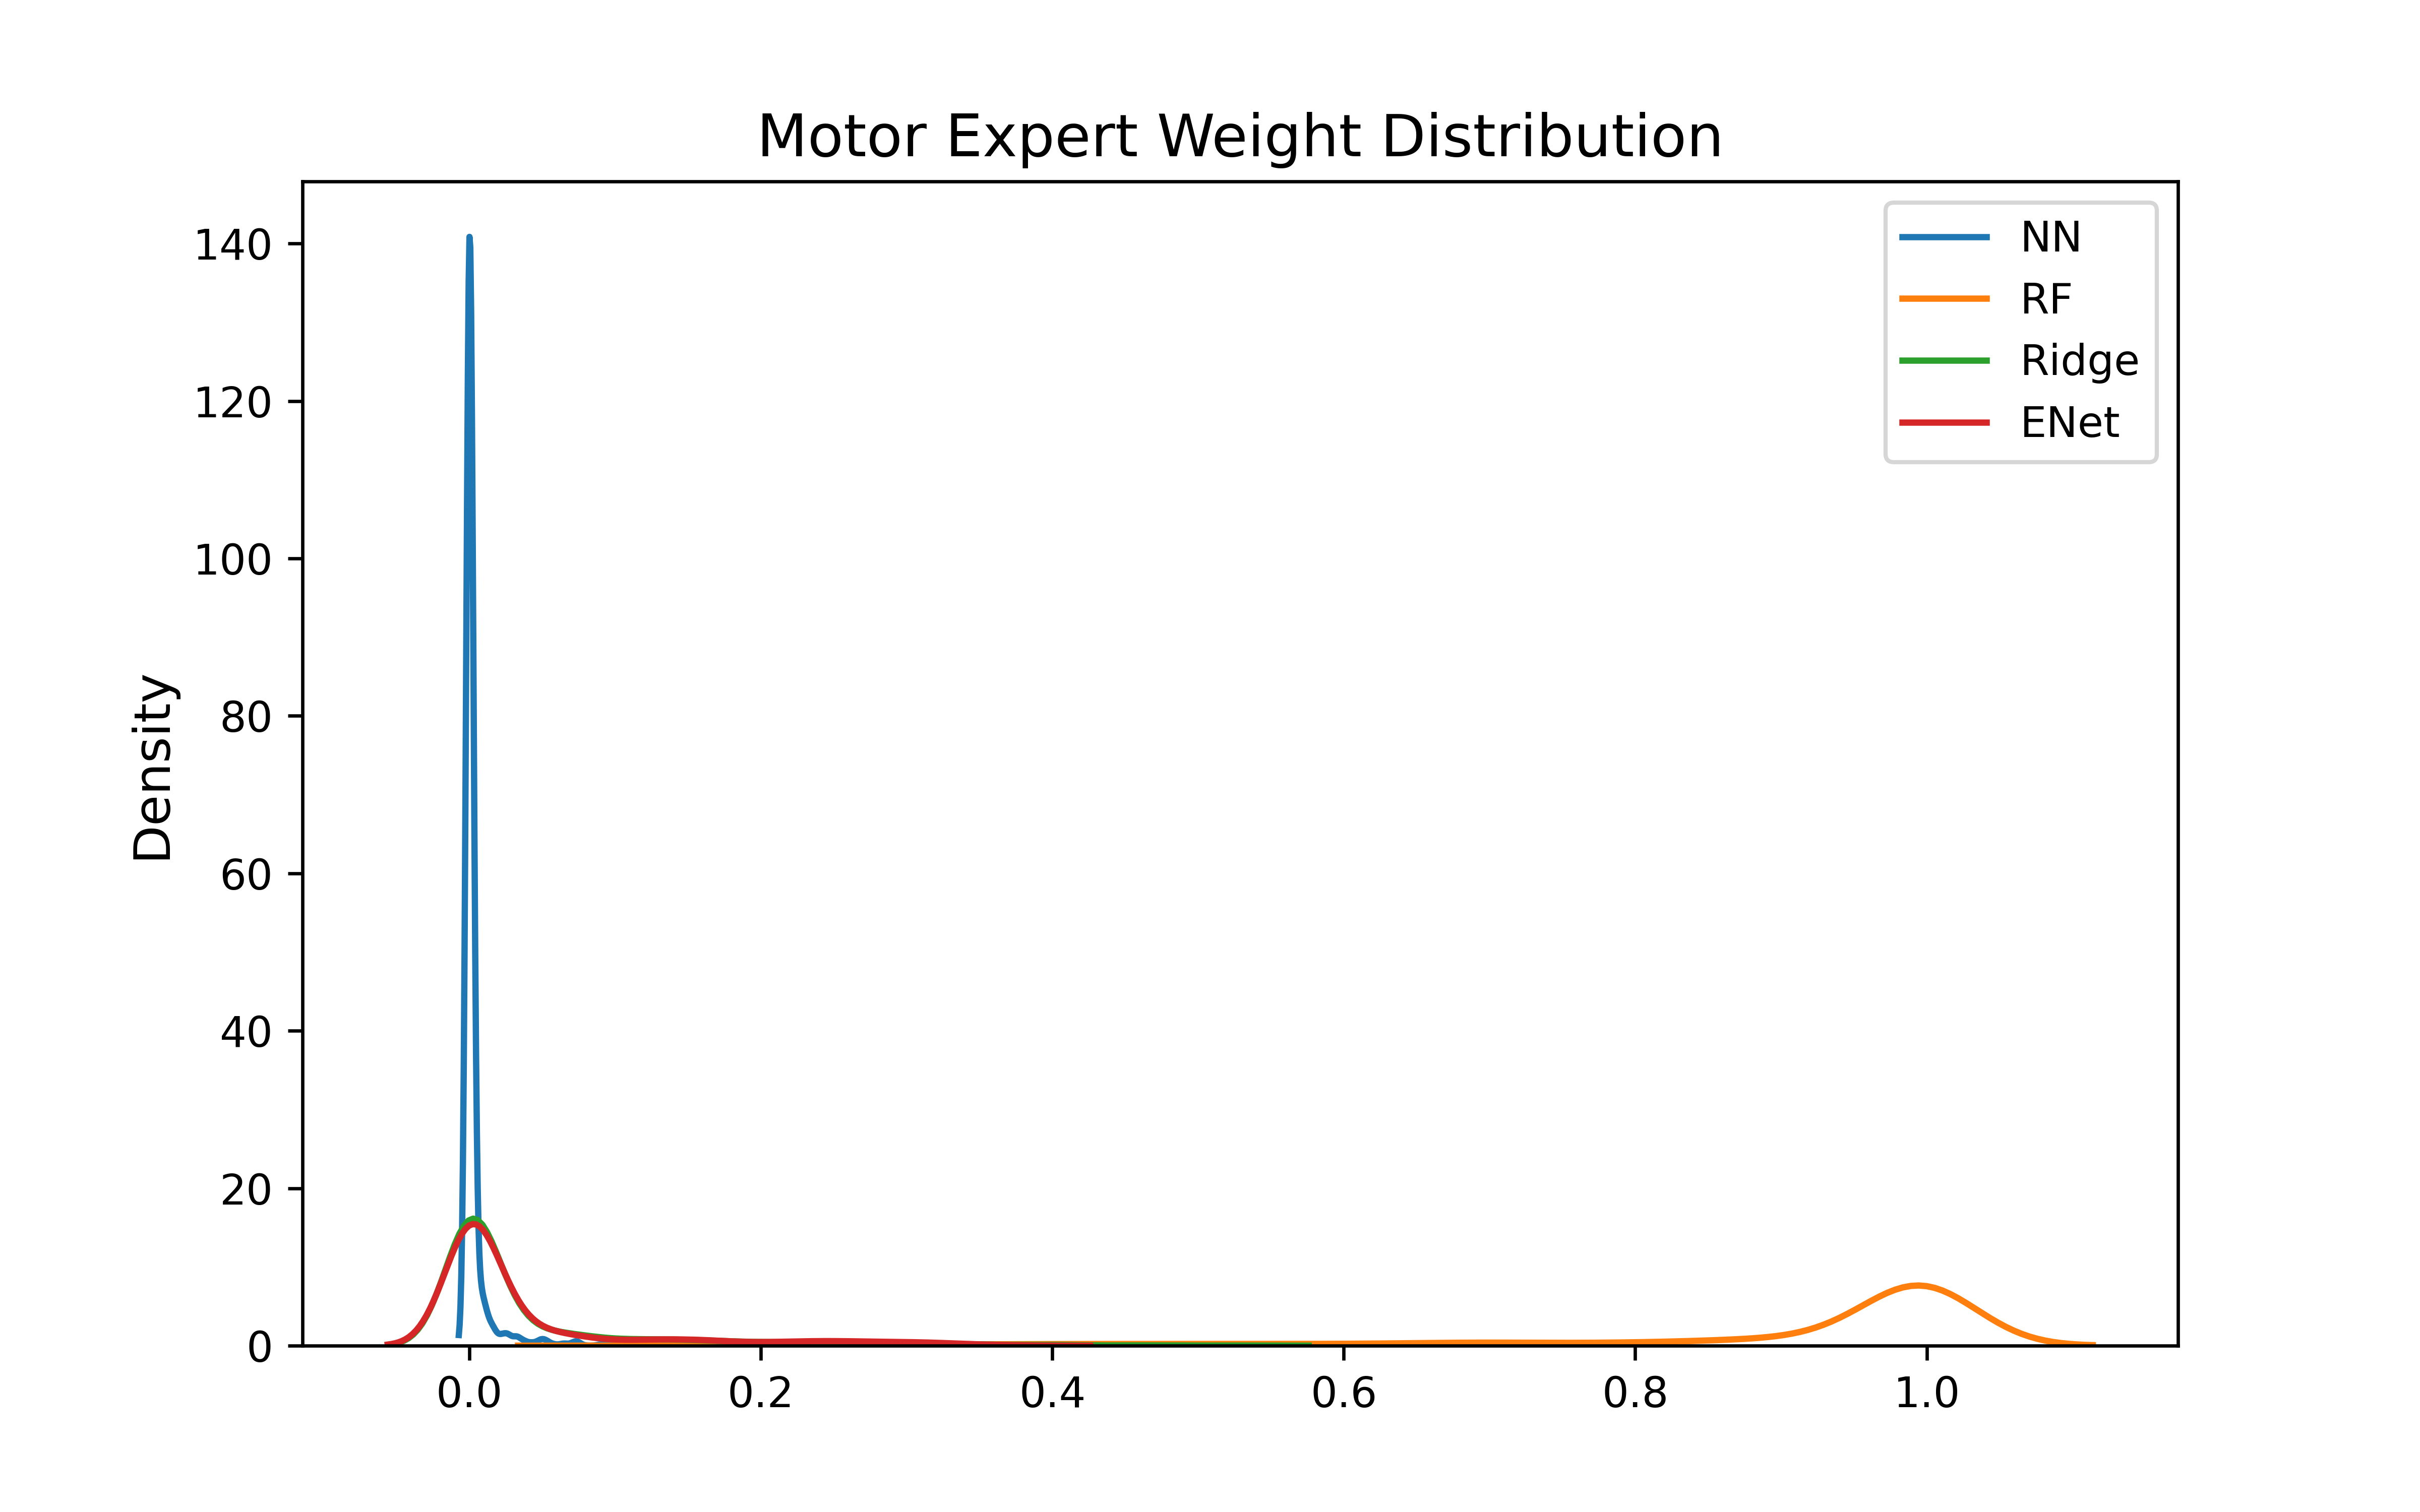
\includegraphics[width=\linewidth]{images/motor_expert_weight_distribution.png}
			\caption{Motor Severity Weights}
		\end{subfigure}
		\hfill
		\begin{subfigure}{0.6\linewidth}
			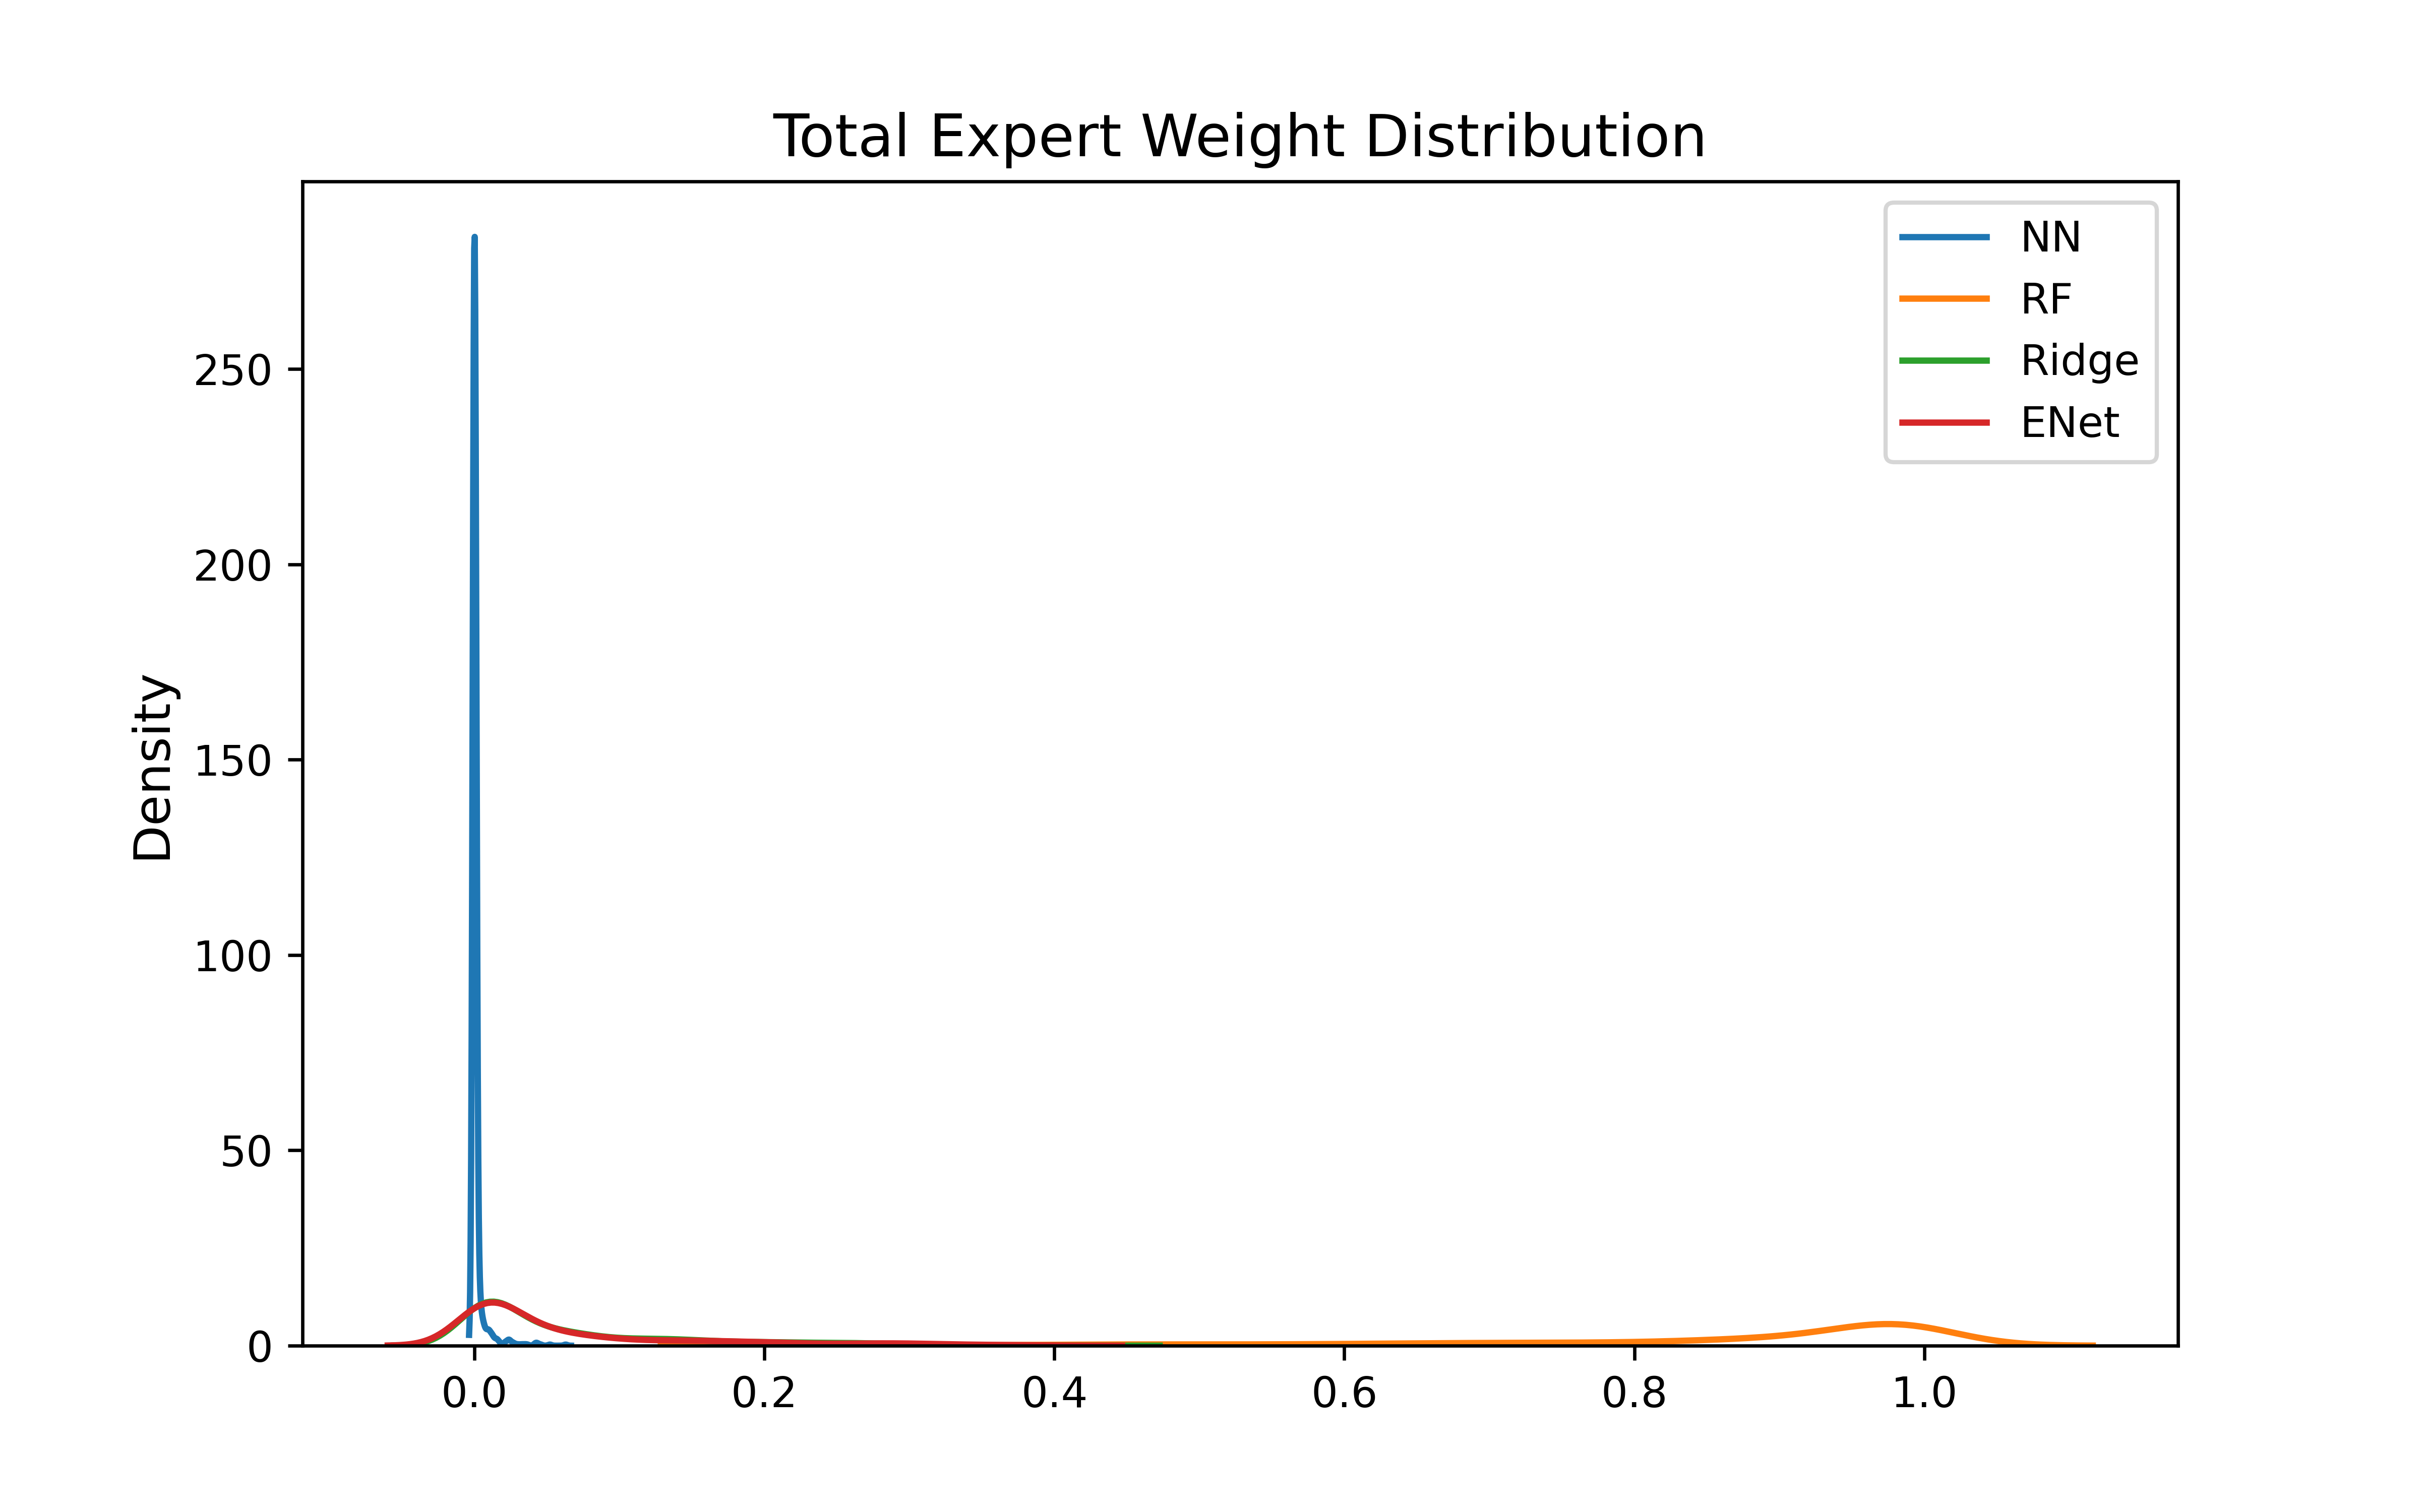
\includegraphics[width=\linewidth]{images/total_expert_weight_distribution.png}
			\caption{Total Severity Weights}
		\end{subfigure}
		
		\caption{Learned expert weight distributions under entropy regularization. The Random Forest expert receives dominant average weight, particularly for motor severity prediction, while total severity exhibits slightly more distributed expert contributions.}
		\label{fig:expert_weights}
	\end{figure}
	
	\section{Discussion}\label{sec:discussion}
	
	The proposed entropy-regularized adaptive Mixture of Experts is competitive in the case of multi-output severity prediction, with an average $R^2$ of 0.9133 on the withheld test data. Although the individual Random Forest has a slight advantage over the MoE using the raw predictive accuracy, the adaptive framework can give further structural information about expert specialization and target-adaptive modeling. Recent surveys highlight how newer models of the Parkinson disease problem are placing greater emphasis on interpretability and robustness, together with predictive behavior, and adaptive ensemble models such as the current one are being encouraged \cite{hossain-2025}.
	
	\subsection{Comparison with Ensemble-Based Regression Models}
	
	In more recent research findings, ensemble method is always found to be superior to individual participants in speech-based Parkinsonism modeling. Shastry illustrated that ensemble regression models are more robust compared to single regressors since diversity in hypothesis enhances stability in prediction in the estimation of UPDRS motor score \cite{shastry-2023}. On the same note, Nilashi et al. showed that the ensemble configurations are more stable in predicting progressions as opposed to the single classifiers \cite{nilashi-2022}.
	
	The usefulness of tree-based heterogeneity is also supported by the findings of Sheikhi and Kheirabadi \cite{sheikhi-2022}, who used a Rotation Forest-based ensemble to predict the severity. Motamedi and Villanyi~\cite{motamedi-2025} also demonstrated that severity estimation is better using hybrid machine learning techniques that use feature optimization and ensemble learning.
	
	These findings are in line with empirical superiority of the Random Forest expert as observed in the present study, which suggests that nonlinear partitioning mechanisms are effective in capturing the complex acoustic-clinical associations between UPDRS estimation.
	
	\subsection{Positioning Relative to Recent Voice-Based Detection Advances}
	
	In addition to other regression-related studies, recent studies have extended speech-based Parkinson modeling to early diagnosis and explainable predictive pipelines. Swain et al.~\cite{swain-2024}emphasized on the role of structured preprocessing and feature engineering in early intervention systems. Neto~\cite{neto-2024} pointed out that voice-based diagnosis is still vulnerable to cross-dataset variability, indicating that adaptive systems that can use a wide range of acoustic distributions are a promising way to go in the future.
	
	Xu et al.~\cite{xu-2025} suggested a speech-based interpretable machine learning framework to detect Parkinson in the speech, with particular focus on clinically clear methods of modeling. Even though their work involves classification tasks, the priority of interpretability is consistent with the direct allocation of expert weights that the entropy-regularized gating mechanism presented in this work allows.
	
	Simone et al.~\cite{simone-2025} also explored the interpretable early detection by analyzing speech, which supports the trend of transparency in biomedical AI. In comparison to post-hoc interpretability frameworks, the existing MoE framework exposes expert insights in the explicit ways of convex weight assignment, which is consistent with larger trends of dispenable clinical AI systems \cite{chaithanya-2025}.
	
	\subsection{Adaptive Architectures and Gating Mechanisms}
	
	The recent neurological modeling studies have been getting more and more adaptive in terms of expert-based design. Mixture of Experts framework proposed by Raza et al.~\cite{raza-2025} to classify multimodal neurological disorder in transformer form is demonstrated to possess scalability, and has the benefit of modular specialization. Titouni et al.~\cite{titouni-2026} proposed a confidence-gated hybrid ensemble to the speech analysis of Parkinson and once again, the use of gating mechanisms to enhance the robustness of the ensemble proved to be essential.
	
	Hadia et al.~\cite{hadia-2025} talked about the concepts of modular deployment of large scale machine learning systems based on MoE architectures with an emphasis on scalability and distributed specialization on complicated data sets. The principles are modified to form structured acoustic regression in the current work, in which entropy regularization prevents expert collapse and promotes even-handed specialization.
	
	Mixture models are very theoretically motivated to be regularized. Khalili and Lin~\cite{khalili-2013} showed that regularization solves degeneracy problems in highly parameterized finite mixture regression models. The results of the experimental expert-weight distributions presented in this paper confirm the perception that entropy regularization is an effective way to avoid trivial expert dominance, and still to permit useful specialization. In addition to statistical regularization, the contextual gating mechanisms have been demonstrated to improve interpretability by training model behaviour on the input properties, in addition to supporting adaptive strategies of expert assignment in structured prediction tasks \cite{al-shedivat-2020}.
	
	
	\subsection{Multi-Output and Personalized Modeling Context}
	
	Combined modeling of correlated clinical outcomes has not been highly achieved in Parkinson disease research using speech. Tong et al. ~\cite{tong-2025} revealed that mixed-effects modeling is better in prediction of progression because it takes into consideration inter-target dependencies. On the same note, Konyar et al.~\cite{konyar-2025} emphasized the significance of personalized multi-task learning to model heterogeneous people with the help of a tensorized representation.
	
	The proposed framework consists of inter-target structure by using two target-specific gating functions with differentiated weight of expert in the $motor\_UPDRS$ and $total\_UPDRS$. The empirical finding that total severity is more weighted to experts indicates that more signals are being integrated in the total as opposed to motor only models of acoustic perturbation.
	
	\subsection{Context within Broader Reviews}
	
	Detailed literature analyses reveal the increasing popularity of ensemble and hybrid machine learning solutions to the study of Parkinson. According to Rabie and Akhloufi~\cite{rabie-2025}, there was fair stability in the performance improvements linked to the ensemble-based detection systems. Shokrpour et al.~\cite{shokrpour-2025} also noted interpretability, generalization and deployment stability as significant open challenges in the field.
	
	Mixture of Experts framework with entropy-regularized directly solves these problems by providing nonlinear predictive robustness to the combination of interpretable adaptive weighting. Although the Random Forest expert is the most powerful standalone predictive signal, the MoE architecture offers a principled control of being able to specialize, predicting accuracy verses the structural transparency.
	
	\section{Limitations of the Study}
	\label{sec:limitations}
	
	Although the suggested entropy-regularized adaptive Mixture of Experts framework is performing well and can be interpreted, there are a number of weaknesses that need to be considered.
	
	To begin with, the research is based on one publicly available voice data, which might not be applicable to generalizing the results to different recording conditions, different languages, and different demographic groups. Microphones MMI can have a considerable effect on speech features, so linguistic variations and clinical heterogeneity can cause significant variations in speech, and thus must be verified externally on independent sets.
	
	Second, despite the interpretable expert weighting that has been offered by the adaptive MoE architecture, the structure still relies on pre-extracted acoustic features as opposed to raw representations of speech. Direct learning of end-to-end models directly based on waveform or spectrogram data can potentially capture more temporal dynamics than a manually-designed pipeline of features can.
	
	Third, although entropy regularization reduces the dominance of experts and encourages equal specialized allocation, the optimal amount of regularization is data-dependent. Automated or theoretically based choice of regularization parameters may also enhance the ability to be robust and minimise manual adaptation.
	
	Lastly, the proposed framework is concerned with severity estimation using regression and does not include longitudinal patient trends. The progression of the PD is time-dependent, and subsequent studies that include sequential or time-conscious learning models would be more precise in describing disease progression.
	
	\section{Future Work}\label{sec:future}
	
	This work has a number of avenues in future research.
	
	To begin with, adaptive specialization and performance can be further improved by joint optimization of experts and gating networks in an end-to-end training framework. It can be enhanced by replacing weak performance in low-confidence prediction areas with uncertainty-sensitive gating mechanisms and Bayesian expert formulations.
	
	Second, the longitudinal modeling strategies can be incorporated to allow progression-sensitive severity prediction over time, which can be used to enhance personalization in chronic disease surveillance.
	
	Third, multimodal biomarkers - gait signals, handwriting dynamics, data collected by wearable sensors, or neuroimaging characteristics - can be integrated into the proposed architecture to expand it into profiling the disease holistically.
	
	Lastly, other MoE variants based on transformers or attention could offer more contextual modeling capacity and also retain adaptive expert specialization.
	
	Such guidelines can help lead to more scalable, interpretable, and clinically dependable AI-assisted systems to monitor the Parkinson disease.
	
	\section{Conclusion}\label{sec:conclusion}
	
	This paper presented an entropy-based regularization adaptive Mixture of Experts (MoE) system to multiplex voice-derived acoustic features prediction of the severity of Parkinson’s disease. The suggested architecture combines heterogeneous expert models - neural, tree-based, and regularized linear regressor - with an expert-specific gating mechanism which dynamically determines convex expert weights between $motor\_UPDRS$ and $total\_UPDRS$ estimation.
	
	Experimental analysis found that the ensemble-based methods are significantly better than the standalone linear methods, which proved that the mapping between acoustic biomarkers and clinical severity is nonlinear and heterogeneous. Although the overall predictive performance of Random Forest was the best, the presented MoE framework showed competitive accuracy with a greater ability to interpret because of clear distributions of weights of experts. Entropy regularization was able to reduce the problem of expert collapse and enhance consistent specialization with varying severity objectives.
	
	The findings support the validity of adaptive ensemble modeling to scalable, non-invasive monitoring of Parkinson disease with telemonitoring voice data. The suggested framework provides flexible and scalable machine-learned basis of resilient severity forecasting within heterogeneous clinical groups.
	
	\section*{Supplementary Materials} \label{sec:supplementary} \addcontentsline{toc}{section}{Supplementary Materials}

Additional experimental visualizations are provided in the supplementary material. These include:

\begin{itemize}
	\item Actual vs. predicted plots for all individual expert models.
	\item Residual distribution analyses for motor and total severity targets.
	\item Error distribution histograms for each expert.
	\item Detailed expert weight distributions for both $motor\_UPDRS$ and $total\_UPDRS$.
\end{itemize}

These supplementary figures provide further insight into model calibration behavior, error dispersion patterns, and adaptive expert specialization dynamics.

	\printbibliography
	
\end{document}